%%%%%%%%%%%%%%%%%%%%%%%%%%%%%%%%%%%%%%%%%%%%%%%%%%%%%%%%%%%%%%%%%%%%%%%%%%
%%%%%                         CHAPITRE 1                            %%%%%%
%%%%%%%%%%%%%%%%%%%%%%%%%%%%%%%%%%%%%%%%%%%%%%%%%%%%%%%%%%%%%%%%%%%%%%%%%%

\lhead[\fancyplain{}{\leftmark}]%Pour les pages paires \bfseries
      {\fancyplain{}{}} %Pour les pages impaires
\chead[\fancyplain{}{}]%
      {\fancyplain{}{}}
\rhead[\fancyplain{}{}]%Pour les pages paires 
      {\fancyplain{}{\rightmark}}%Pour les pages impaires \bfseries
\lfoot[\fancyplain{}{}]%
      {\fancyplain{}{}}
\cfoot[\fancyplain{}{\thepage}]%\bfseries
      {\fancyplain{}{\thepage}} %\bfseries
\rfoot[\fancyplain{}{}]%
     {\fancyplain{}{\scriptsize}}


%%%%%%%%%%%%%%%%%%%%%%%%%%%%%%%%%%%%%%%%%%%%%%%%%%%%%%%%%%%%%%%%%%%%%%%%%%
%%%%%                      Start part here                          %%%%%%
%%%%%%%%%%%%%%%%%%%%%%%%%%%%%%%%%%%%%%%%%%%%%%%%%%%%%%%%%%%%%%%%%%%%%%%%%%

\chapter{Contexte industriel et objectif de recherche}
\label{ch:objectives}

%==============================================================================	Résumé du chapitre

\begin{center}
\rule{0.7\linewidth}{.5pt}
\begin{minipage}{0.7\linewidth}
\smallskip

\textit{
Dans ce premier chapitre, nous présentons le contexte du procédé d'injection-moulage des thermoplastiques dans lequel s'inscrit nos travaux.
Dans un premier temps, nous étudierons l'état de l'art de la maîtrise de la qualité en injection-moulage.
Dans un second temps, nous identifions les verrous au déploiement du contrôle de la qualité à cent pourcent.
Enfin, nous présentons nos objectifs de recherche pour les lever.
}

%\smallskip
\end{minipage}
\smallskip
\rule{0.7\linewidth}{.5pt}
\end{center}

\minitoc
\newpage

\section{Le procédé d'injection-moulage des thermoplastiques}  \label{sec:molding_presentation}
Notre travail s'inscrit dans le cadre du projet de recherche collaboratif FUI SAPRISTI, qui cherche à optimiser le procédé d'injection-moulage des thermoplastiques.
Dans cette première section, nous présenterons ce procédé de mise en forme des pièces par moulage d'un thermoplastique.
% Dans cette section, nous présentons le fonctionnement du procédé d'injection-moulage.

% \subsection{Présentation du procédé d'injection-moulage des thermoplastiques}
La machine qui met en œuvre le procédé d'injection-moulage est la presse à injecter.
Un polymère est fondue dans un tube (appelé le "fourreau") chauffé.  % est au dessus de son point de fusion qui 
Le fourreau contient une vis pour malaxer la matière.  % et la "plastifier".
La rotation et l'avance de la vis sont régulées afin de définir les caractéristiques de la matière fondue qui sera injectée.
En particulier, il s'agit d'homogénéiser la matière fondue afin qu'elle ait une certaine viscosité.
L'avancée de la vis produit une pression sur la matière qui est également régulée : c'est la pression d'injection.
Le procédé d’injection-moulage des thermoplastiques consiste à injecter sous une pression élevée (pression > 100 MPa) le polymère fondu (température > 200°C) et visqueux dans un moule.
La pression est maintenue pendant le refroidissement de la matière ; en particulier jusqu'à ce que le canal par lequel la matière est entrée dans le moule soit solidifié.
Cette phase de maintien permet de compenser le retrait de la matière consécutif à sa solidification.
Le passage de la phase de maintien à la phase d'injection est appelé la commutation (on parle couramment de "point de commutation").
L'ensemble qui constitue le moule est appelé un "outillage" ; ce dernier intègre un système de régulation thermique afin de favoriser le refroidissement de la pièce.
L'outillage doit également supporter les contraintes mécaniques des pressions d'injection et l'on cherche à éviter la déformation de sa géométrie pendant l'injection.
De manière générale, les outillages en injection-moulage sont volumineux et massifs et comparaison des dimensions des pièces produites.

\begin{figure}[hbtp]
	\centering
	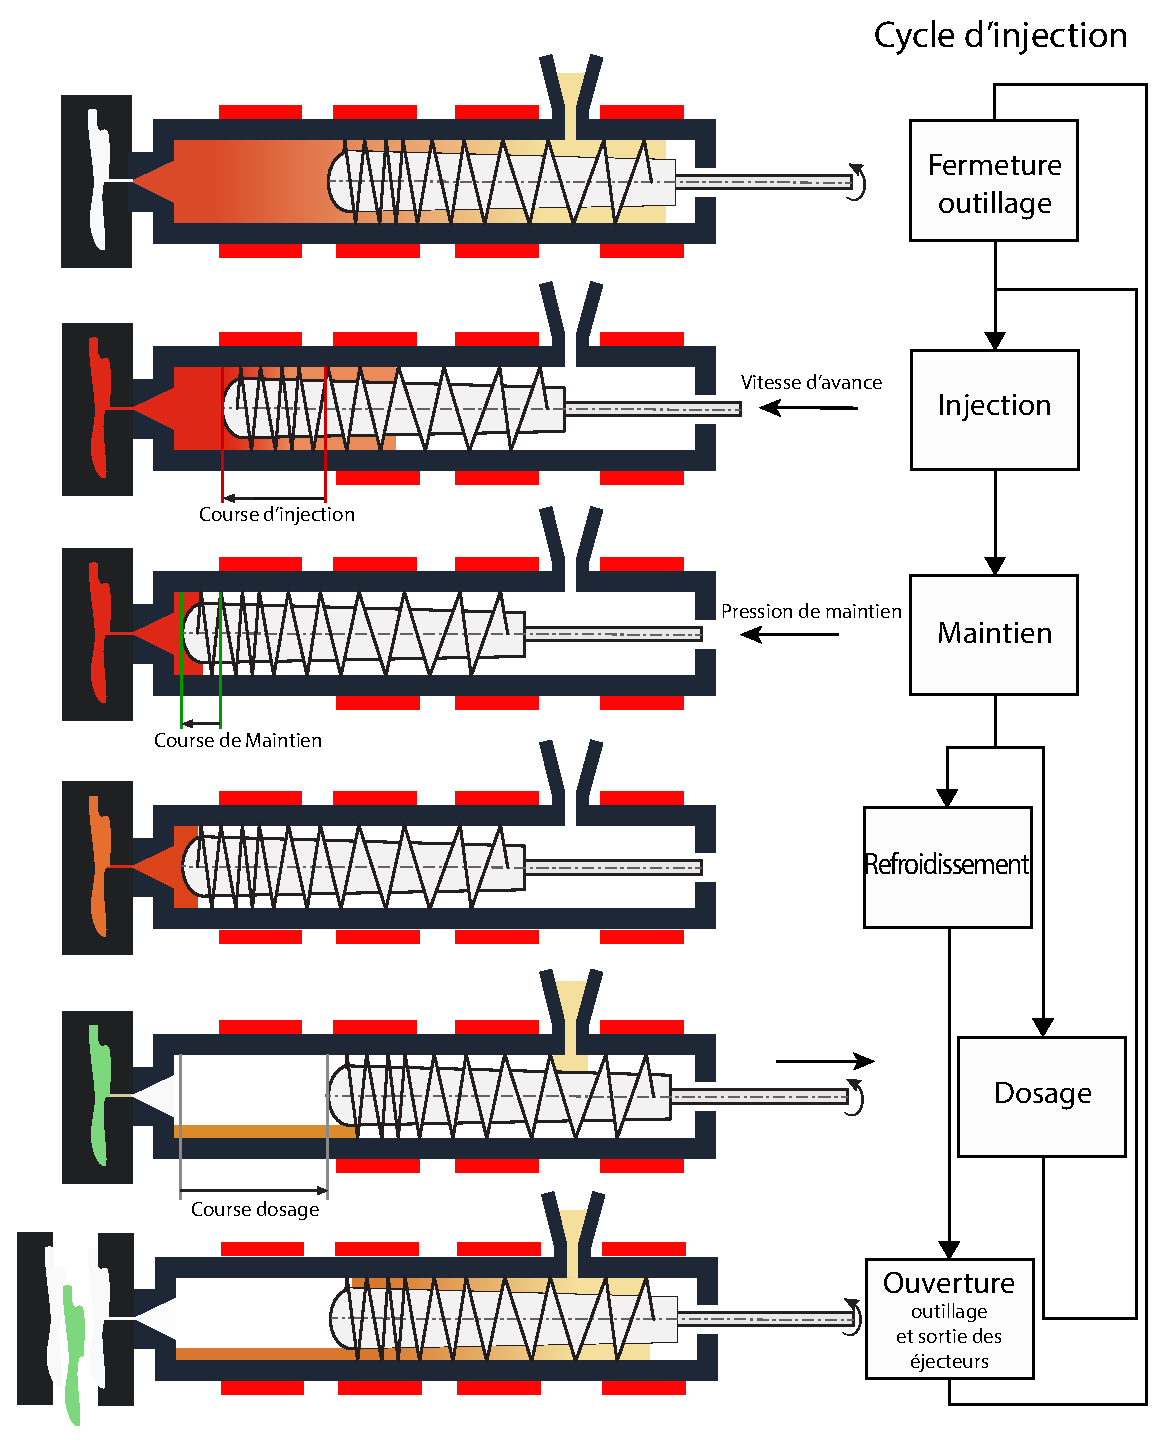
\includegraphics[width=0.9\textwidth,height=\textheight,keepaspectratio]{../Chap1/Figures/SAPRISTI_Schema-cycle.pdf}
	\caption{Schéma-bloc du procédé d'injection-moulage.}
	\label{fig:cycle_injection}
\end{figure}

Le procédé d'injection-moulage des thermoplastiques est un procédé cyclique.
Afin de mettre en évidence la séquence d’un cycle du procédé, nous proposons un schéma bloc d’un cycle d’injection, voir la Figure \ref{fig:cycle_injection}.
On remarque en particulier que l'étape de dosage est réalisé en parallèle du refroidissement de la pièce et de son éjection.
Le dosage est l'étape où la matière première est fondue dans la vis d'injection.
C'est une étape clé car il est nécessaire de garantir une certaine viscosité de la matière fondue.
À cause de l'étape de dosage, la production d'une pièce est conditionnée par la production de la pièce précédente.
Lors du démarrage d'une presse à injecter, il est courant de produire une vingtaine de pièce pour ajuster les réglages et stabiliser le cycle.
Nous détaillons dans la Section \ref{subsec:process_parameters} suivante les paramètres qui peuvent être réglés sur une presse à injecter.

Le procédé d'injection-moulage est également séquentiel : il est composé de phases successives.
Chaque phase possède des paramètres qui influent sur les phases suivantes et, à terme, sur les caractéristiques du produit fini.
Les multiples phases font que le nombre de paramètres qui peuvent être ajustés sur le procédé est grand (> 20).
Il est possible d’ajuster précisément les températures, les courbes de pressions et les durées d’ouvertures et de fermetures de multiples buses d’injection.
% Ainsi, l’espace des variables de pilotage est grand et les variables sont continues.
Enfin, le procédé d'injection-moulage possède une certaine inertie : c'est à dire que l'ajustement d'un des paramètres du procédé met une certaine durée avant de se répercuter sur la production.
Cette inertie est majoritairement due à l'inertie thermique de l'outillage massif.

% refroidi ; à maintenir une pression de compactage pendant une durée spécifique; puis à éjecter la pièce tout en préparant en parallèle la matière nécessaire au cycle suivant. 

% Relecture Éric
% Présenter les contraintes du procédé d'injection
% -> Réglage initial du point de fonctionnement difficle
% -> Peu de dérive du procédé, causes exceptionnelles de Shewart
% -> Pas ou peu de mesure de la qualité en ligne de production, pourquoi ? -> introduire notre travail

D'un point de vue industriel, l’injection-moulage des thermoplastiques est un procédé à haute cadence, peu coûteux car répétable.
Une fois la presse à injecter réglée, le procédé est généralement stable dans le temps.
Il peut produire de manière continue plusieurs milliers de pièces sans intervention humaine.
De plus, le coût de la matière première thermoplastique est faible.

La pratique industrielle de la production d'une pièce par moulage de thermoplastique suit généralement la séquence suivante :
\begin{enumerate}
	\item Apport de la matière première
	\item Injection-moulage de la pièce
	\item Stockage des pièces
	\item Étapes de finition (traitements de surface, peintures) 
	\item Stockage des pièces
	\item Contrôle de la qualité
	\item Expédition
\end{enumerate}
Le contrôle de la qualité des pièces n'est aujourd'hui pas réalisé dès la sortie du moule (après l'étape 2.).
Ainsi, si une pièce est non-conforme dès l'étape d'injection-moulage, elle ne sera pas écartée de la chaîne de production.
Nous discuterons en particulier dans la Section \ref{sec:research_objectives} des limites qui s'opposent à la réalisation du contrôle en ligne de production.
% ; puis nous présenterons les objectifs de recherche de notre travail de doctorat concernant ce point.

\subsection{Paramètres réglables d'une presse à injecter} \label{subsec:process_parameters}
Le nombre de paramètres réglables d'une presse à injecter est grand.
Dans le Tableau \ref{tab:process_parameters}, nous répertorions les 16 paramètres les plus courants qui peuvent être réglés sur un presse.
Cette liste n'est pas exhaustive.
En particulier, les choix de la matière première, de la buse et les profils d'évolution des pressions ajoutent de nombreuses possibilités de réglages.

Nous remarquons que de nombreux paramètres sont dépendants.
Par exemple, les vitesses dépendent de la durée du cycle que l'ont souhaite obtenir.
La pratique industrielle du procédé d'injection-moulage fait appelle au savoir-faire du technicien pour régler le point de fonctionnement initial.
Sur des pièces compliquées, le réglage du procédé peut prendre plusieurs heures.

\begin{table}[bhtp]
	\centering
	\arrayrulecolor{black}
	\hspace*{-14mm}
	\begin{tabular}{|llll|}
		\arrayrulecolor{black}
		%\cline{1-1} \cline{3-6}
		\hhline{----}
		Phase du procédé & Paramètres réglables & Description & Valeur classique \\ \hhline{=:=:=:=:} %\hline
		Dosage                   & Course de dosage                 & Distance d'avance de la vis                                                    & 50-100 cm                      \\
		Dosage                   & Température du fourreau          & Températures des colliers chauffants                                   & 200-300 °C                     \\
		Dosage                   & Vitesse de rotation de la vis    & Rotation de la vis qui malaxe la matière                                                      & 1-20 tours/min                 \\
		Injection                & Course d'injection               & Distance d'avance de la vis pendant l'injection                                               & 50-100 cm                      \\
		Injection                & Pression d'injection             & Profil de pression exercée sur la vis                            & 10-200 MPa                     \\
		Injection                & Pression de commutation          & Détermine le passage de l'injection au maintien & 10-100 MPa                     \\
		Injection                & Vitesse d'injection              & Vitesse d'avance de la vis                                                & 0,5 - 1 m/s                    \\
		Maintien-refroid. & Durée de maintien                & Durée de maintien de la pression                                                & 10-60 s                        \\
		Maintien-refroid. & Pression de maintien             & Profil de pression exercée sur la vis                            & 10-100 MPa                     \\
		Maintien-refroid. & Débit thermorégulateur           & Débit de circulation du fluide                    & 20-100 dm$^3$/s \\
		Maintien-refroid. & Température thermorégulateur     & Régulation thermique du moule                           & 10-40 °C                       \\
		Ouverture-éjection     & Course d'ouverture               & Distance d'ouverture de l'outillage                                       & 10-100 cm                      \\
		Ouverture-éjection     & Vitesse d'ouverture              & Vitesse d'ouverture de l'outillage                                        & 0,5 - 2 m/s                    \\
		Ouverture-éjection     & Course des éjecteurs             & Distance de sortie des éjecteurs                                      & 1-20 cm                        \\
		Ouverture-éjection     & Vitesse de rentrée des éjecteurs & Vitesse de sortie des éjecteurs                                                               & 0,5 - 2 m/s                    \\
		Fermeture outillage      & Vitesse de fermeture             & Vitesse de fermeture de l'outillage                                                           & 0,5 - 2 m/s                   \\
		\hline
	\end{tabular}%
	\caption{Paramètres réglables sur une presse à injecter classique.}
	\label{tab:process_parameters}
\end{table}


\section{Enjeux de la recherche sur le procédé d'injection-moulage}  \label{sec:research_topics}
Le projet de recherche collaboratif FUI SAPRISTI a pour objectif de limiter la production de pièces non-conformes.
Ce procédé est l'étape clé du processus de fabrication des pièces plastiques moulées.
Il répercute ses défauts sur l'ensemble de la chaîne de production, comme par exemple sur les étapes d'assemblages et les finitions.

Dans cette section, nous identifierons les principaux axes de recherche qui lui sont associés : la modélisation mathématique du procédé, la maîtrise du point de fonctionnement et l'optimisation des réglages.
Enfin, nous discuterons de l'intérêt de notre travail sur le contrôle de la qualité en ligne, dans une perspective de surveillance et de pilotage du procédé.

\subsection{Cartographie bibliographique} \label{subsec:injection_research}
Afin d'identifier les thématiques de recherche qui sont associées au procédé d'injection-moulage, nous avons réalisé une cartographie bibliographique dans la communication \citetitle{nagorny_injection_2017} \cite{nagorny_injection_2017}.
% \subsection{Revue bibliographique sur le procédé d'injection-moulage des thermoplastiques}
% Dans cette section, nous identifierons les principaux axes de recherche qui lui sont associés : la modélisation mathématique du procédé, la maîtrise du point de fonctionnement et l'optimisation des réglages.

\begin{figure}[bhtp]
	\centering
	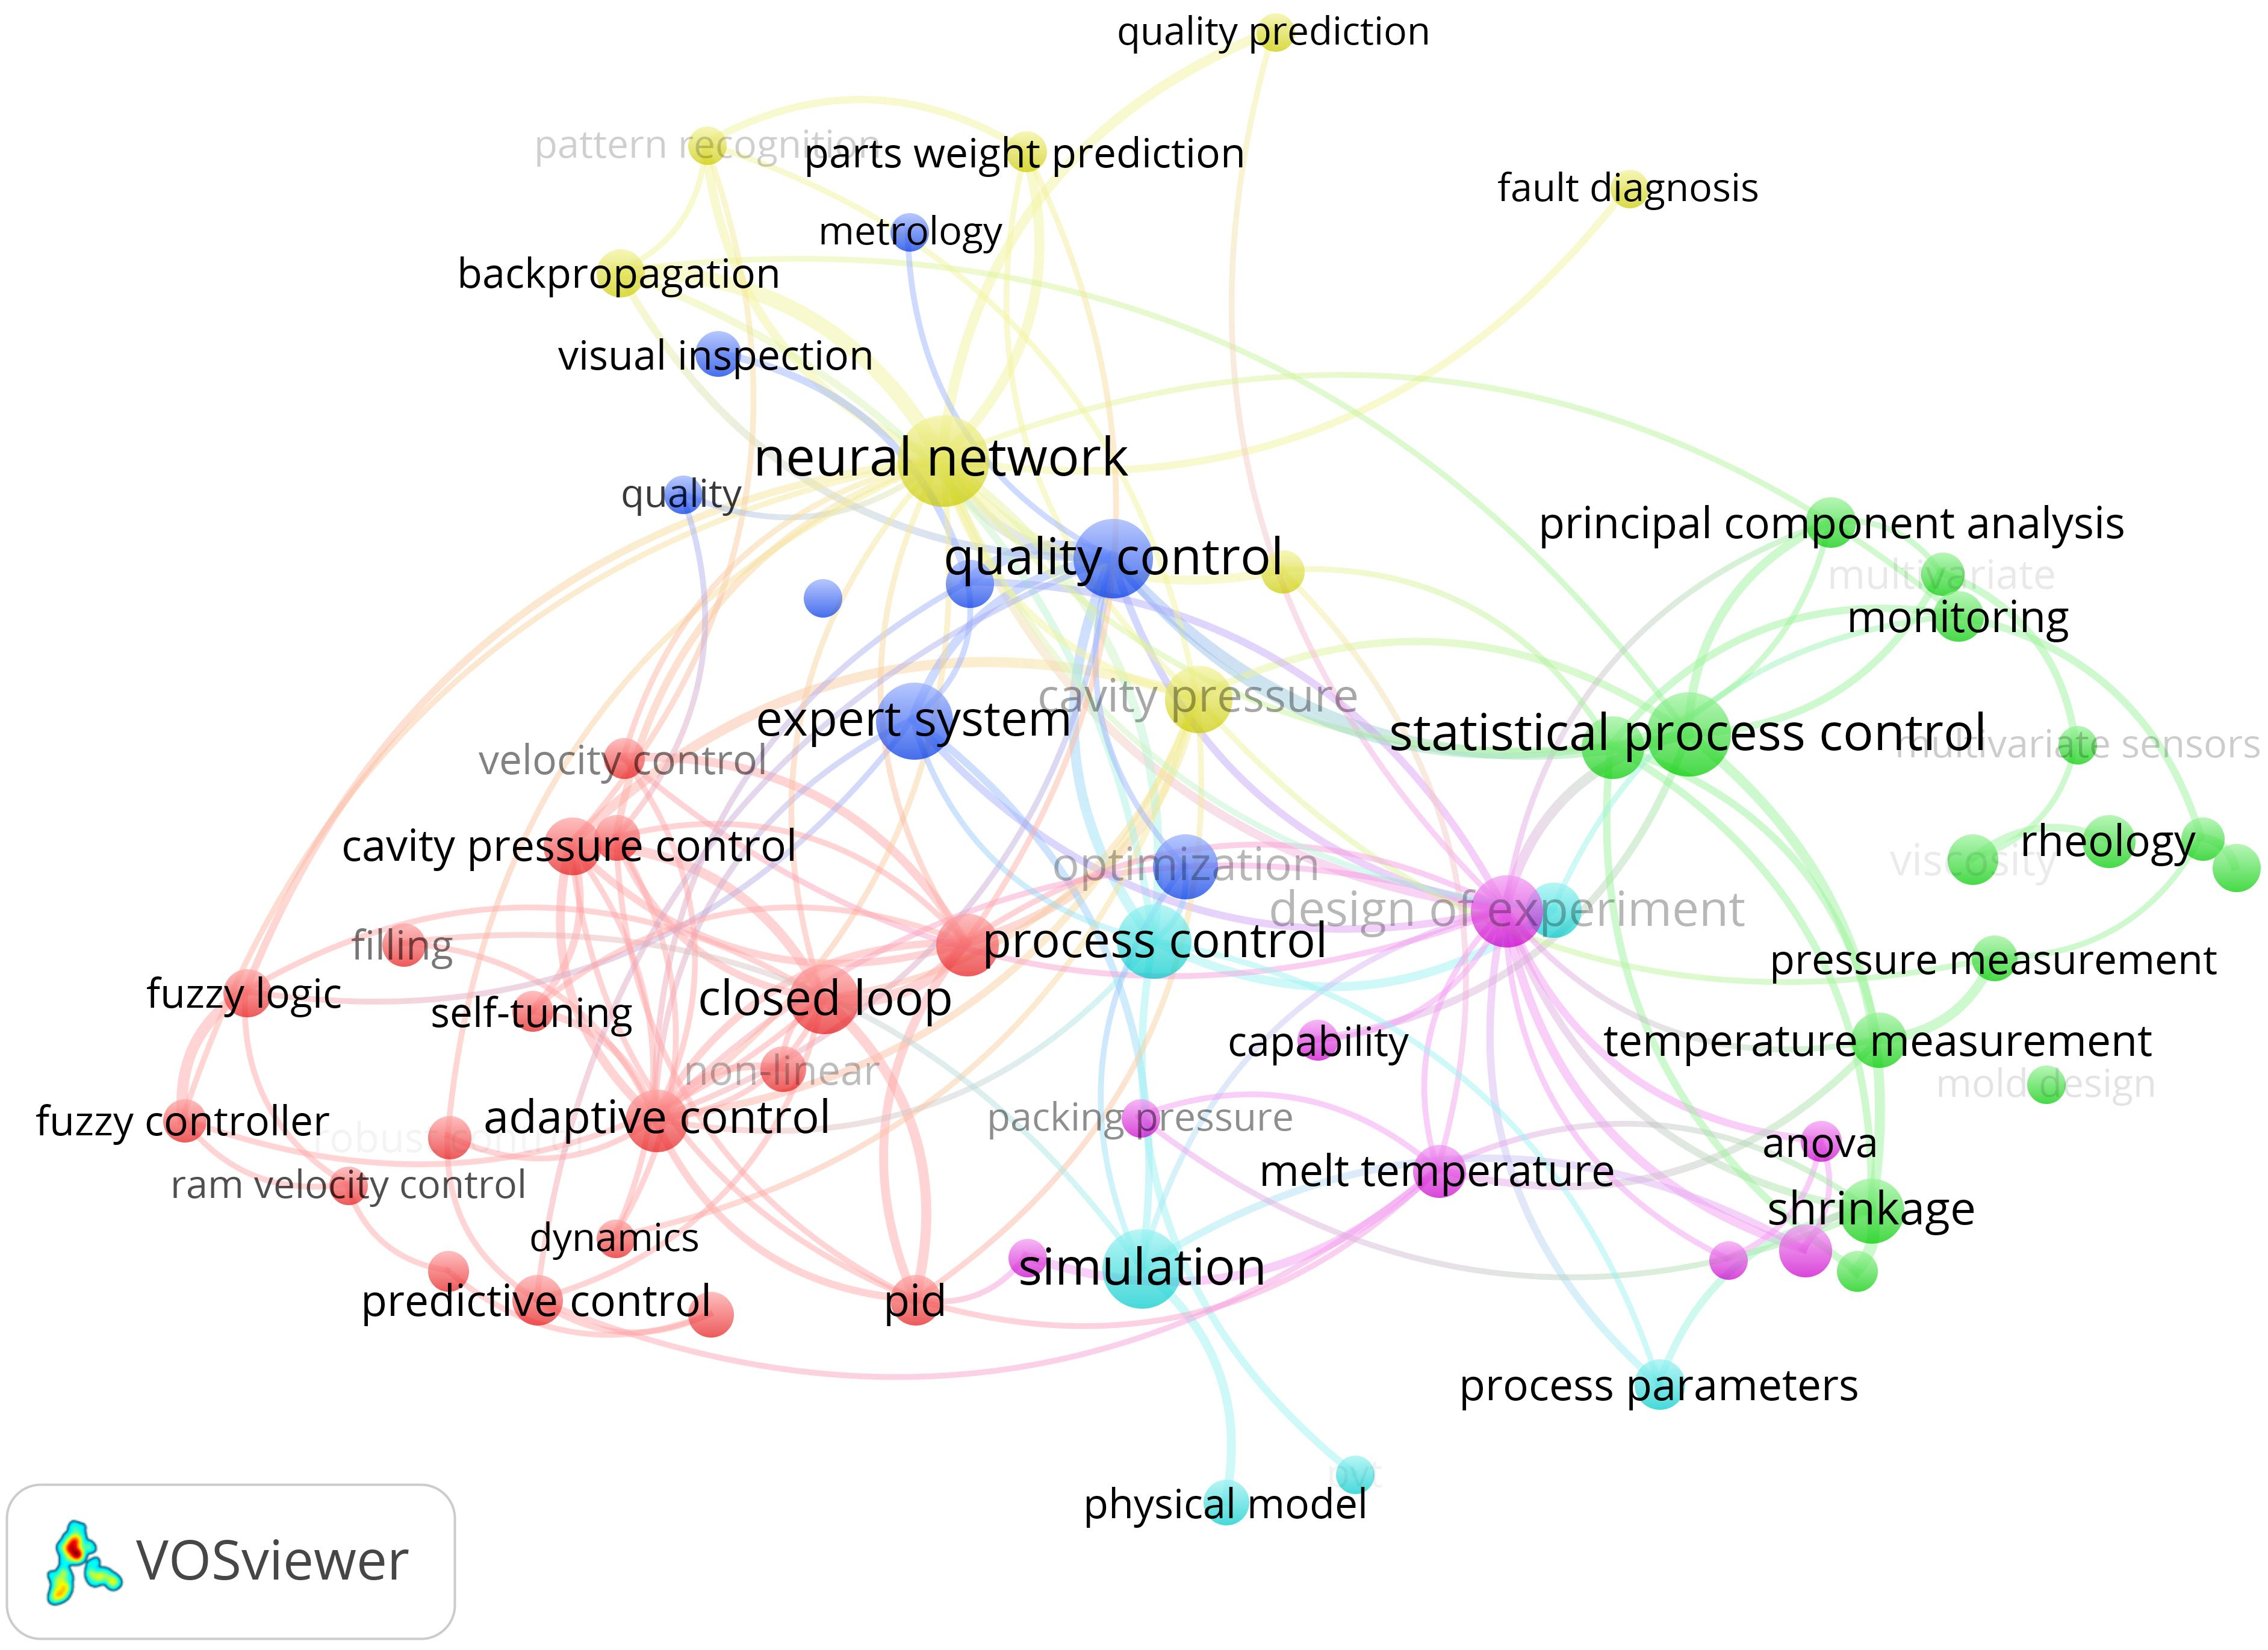
\includegraphics[width=\textwidth,height=\textheight,keepaspectratio]{../Chap1/Figures/tagMapFinalPubliOccurence.jpg}
	\caption{Cartographie bibliographique de la maîtrise du procédé d'injection-moulage.}
	\label{fig:cartographie}
\end{figure}

La Figure \ref{fig:cartographie} présente le graphe relationnel que nous avons construit à partir des mots-clés associés à 421 publications, de 1970 à 2015.
Les mots-clés sont retenus s’ils apparaissent plus de quatre fois.
Ils sont regroupés par relations.
Nous utilisons le formalisme \textit{VOS} (\textit{Visualization Of Similarities}) proposé par \citeauthor{vaneck_vos_2006} \cite{vaneck_vos_2006, van_eck_comparison_2010}.
Sur ce graphique, nous identifions plusieurs thématiques de recherche.
Dans la suite de cette section, nous présenterons chacune de ces thématiques.

\begin{itemize}
	\item la modélisation mathématique et la simulation du procédé (couleur cyan) §\ref{subsubsec:molding_theory},
	\item la modélisation empirique par plan d'expériences (couleur rose) §\ref{parag:molding_doe},
	\item l’apport des systèmes à réseaux des neurones pour modéliser le procédé (jaune) §\ref{parag:molding_neural},
	\item l’apport des systèmes experts pour régler le point de fonctionnement initial (bleu) §\ref{subsec:process_control},
	\item la régulation du point de fonctionnement par l'automatique (couleur rouge) §\ref{subsec:process_control},
	\item l’analyse phénoménologique par la statistique afin de détecter les dérives (vert) §\ref{subsec:process_control}.
\end{itemize}

% Dans la littérature, les réseaux de neurones sont utilisés pour modéliser le procédé de manière empirique.
% La littérature propose de réguler les paramètres du procédé d’injection à partir de la prédiction de caractéristiques des pièces.
% La prédiction à partir de variables du procédé est préférée à une mesure directe sur la pièce, car la métrologie n’est pas assez développée pour permettre une mesure pièce à pièce en cycle industriel.
% À contrario, l'enregistrement des mesures de pression pendant le cycle est très répandue, car elle est implémentée par les fabricants de moules et les fabricants de systèmes de régulations du procédé.
% Enfin, nous distinguons (de couleur rouge) les efforts pour la régulation du procédé.
% De nombreuses méthodes ont été étudiées et nous remarquons l’intérêt porté aux méthodes adaptatives.
% Cependant, chacune de ces méthodes ne s’intéressent qu’à un nombre limité de variables du procédé et des caractéristiques du produit.
% Enfin, l'analyse statistique est utilisée pour détecter les dérives et les défaillances du procédé.
% Elle s’appuie sur la mesure \textit{in-situ} de variables du procédé, parmi lesquelles les plus utilisées sont la température et la pression.
% Ce graphique n'inclut pas les dates des publications.
% Nous invitons le lecteur à consulter notre Tableau récapitulatif \ref{tab:state_art_compare}.
\noindent
L'ensemble de ces travaux de recherche à deux grands objectifs :
\begin{itemize}
	\item améliorer la modélisation du procédé,
	\item maîtriser les caractéristiques des produits fabriqués par le procédé.
\end{itemize}
Ces deux objectifs sont souvent traités de manière complémentaire.
L'amélioration de la modélisation permet une meilleur maîtrise des caractéristiques du produit.
Dans les sections suivantes, nous présenterons chacune des thématiques de recherche que nous avons identifiées.

\subsection{Modélisation du procédé d'injection-moulage}
Le moulage par injection-plastique est un procédé séquentiel qui peut être décomposé en plusieurs phases interdépendantes.
Chacune des phases influe sur la suivante et, à terme, conditionne les caractéristiques du produit.
Nous étudierons puis nous proposerons un modèle systémique du procédé.
Puis nous présenterons les travaux sur les modèles théoriques du procédé d'injection-moulage et les travaux d'identifications de modèles à partir de mesures expérimentales.

\subsubsection{Modélisation systémique} \label{subsubsec:molding_systemic}
En 1999, \citeauthor{kazmer_towards_1999} proposent un découpage en cinq phases \cite{kazmer_towards_1999}, voir la Figure \ref{fig:kazmer_systematic}, qui est une évolution du découpage en trois phases qui avait été proposé par \citeauthor{ma_design_1974} \cite{ma_design_1974}.
Cette représentation systémique du procédé fait apparaître des variables d’état intermédiaires qui sont associées à chacune des phases.

\begin{figure}[bthp]
	\centering
	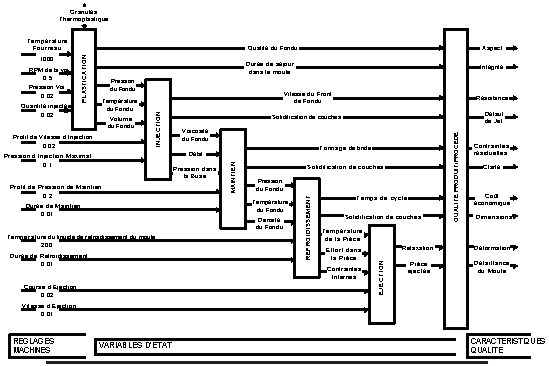
\includegraphics[width=\textwidth,height=\textheight,keepaspectratio]{../Chap1/Figures/Kazmer_1999-Process.pdf}
	\caption{Vue systémique du procédé d'injection-moulage, traduite de \citeauthor{kazmer_towards_1999} \cite{kazmer_towards_1999}.}
	\label{fig:kazmer_systematic}
\end{figure}

Elle fait également apparaître les relations de dépendance entre les différentes phases.
% Les phases sont la cause des caractéristiques du produit.
La représentation met en évidence plusieurs variables intermédiaires, qui influent soit directement sur les caractéristiques du produit, soit sur les caractéristiques d'autres phases.
Ces variables intermédiaires ne sont pas nécessairement observables.
Il est par exemple très difficile de mesurer la densité de la matière fondue, ou bien l'évolution des contraintes internes.

Cette figure permet de mettre en évidence 10 caractéristiques du produit qui sont la cause de 12 variables de réglages.
L'injection-moulage est un procédé multi-entrées, multi-sorties.
On distingue également deux réglages de "profils".
Un profil est une valeur de réglage qui évolue dans le temps.
Aussi, les possibilités de réglages d'un profil sont bien plus importantes que pour un grandeur scalaire : un profil est au minimum composé de 10 points ; nous obtenons alors ici 22 variables de réglages pour 2 profils.
% La modélisation d'un tel procédé est compliquée.
% C'est pourquoi la littérature est riche en modèles empiriques, car les modèles théoriques sont difficiles à réaliser.

\begin{figure}[bthp]
	\centering
	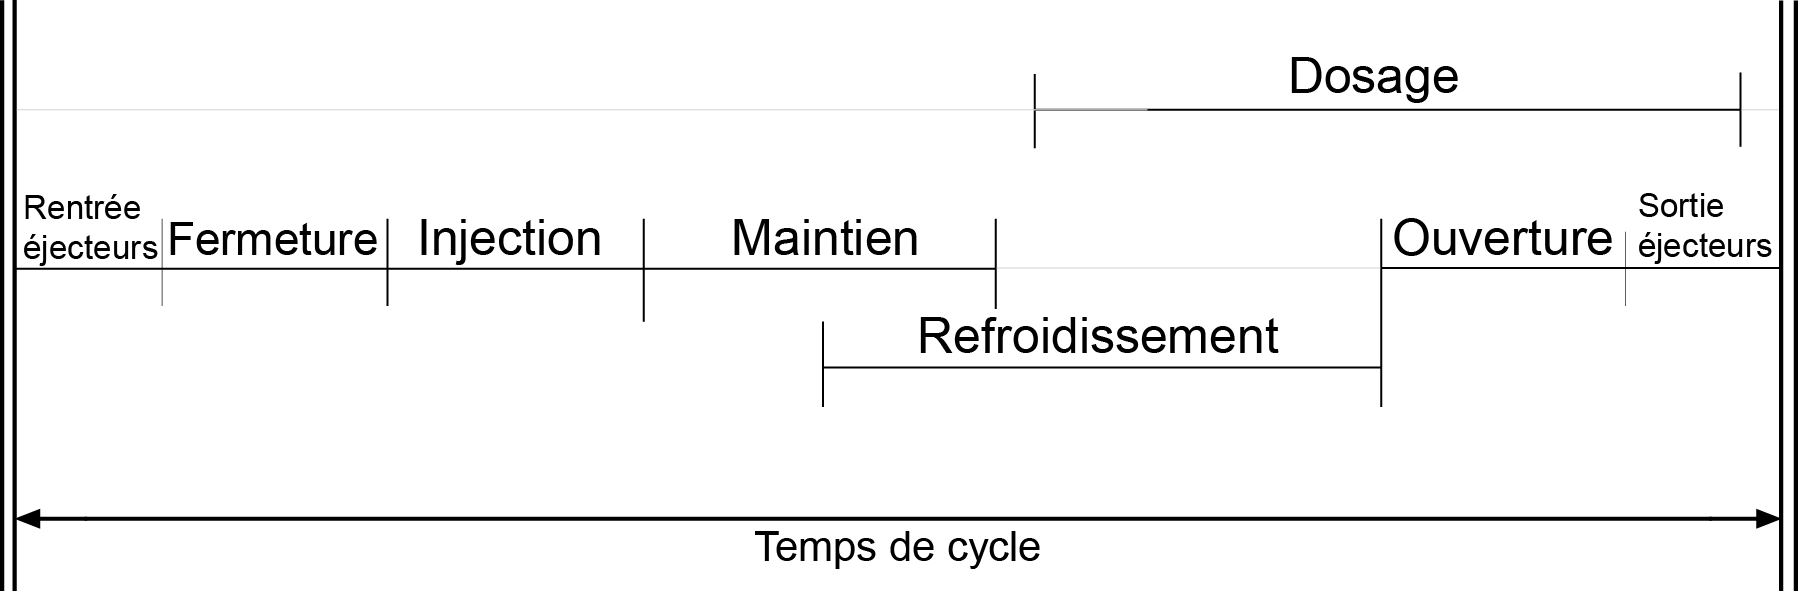
\includegraphics[width=0.82\textwidth,height=\textheight,keepaspectratio]{../Chap1/Figures/SAPRISTI_Chronogramme-Simple.png}
	\caption{Chronogramme du cycle d'injection-moulage.}
	\label{fig:chronogramme}
\end{figure}

Enfin, nous remarquons que cette représentation systémique ne fait par apparaître la nature cyclique du procédé.
C'est pourquoi nous proposons un chronogramme du cycle d’injection : la Figure \ref{fig:chronogramme} représente le caractère cyclique du procédé, en particulier pour l'étape de dosage.
En effet, la phase de dosage est réalisée en temps masqué par rapport à l'ouverture et la fermeture du moule.
Dans une presse à injecter, on distingue deux parties cinématiques indépendantes : la vis de dosage et l'outillage amovible.
Généralement, la phase de dosage débute pendant le refroidissement de la matière, dès que le canal d’alimentation est solidifié.
Elle se termine avant le début de la phase d'injection.
La phase de dosage, qui est réalisée pendant le moulage d'une pièce, conditionne les caractéristiques de la matière fondue pour la pièce suivante ; il y a un cycle de décalage.

\begin{figure}[hbtp]
	\centering
	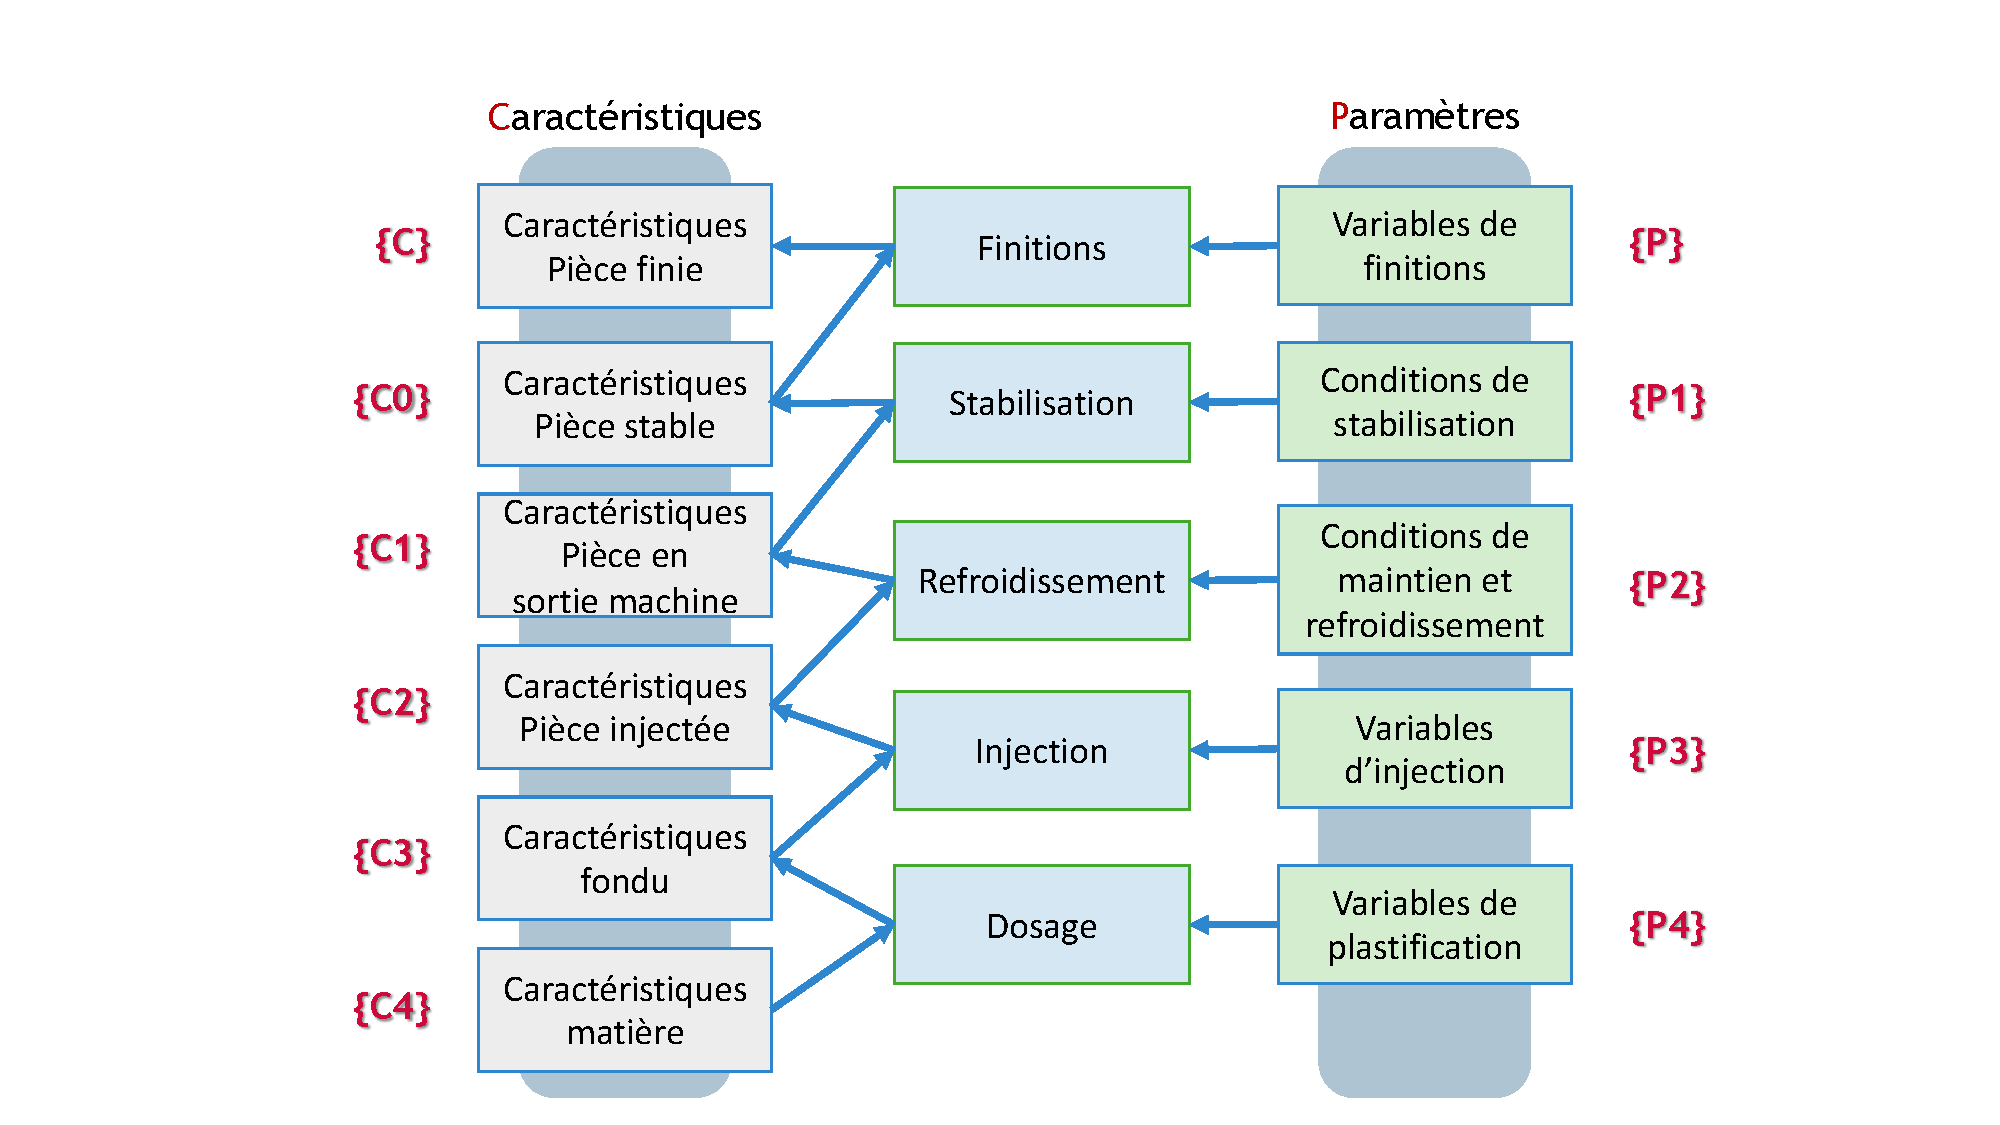
\includegraphics[width=0.85\textwidth,height=\textheight,keepaspectratio]{../Chap1/Figures/Sapristi_ZigZag.pdf}
	\caption{Représentation \textit{Zig Zag} du procédé d'injection-moulage des thermoplastiques.}
	\label{fig:zigzag}
\end{figure}

Dans la Figure \ref{fig:zigzag}, nous proposons une représentation \textit{Zig Zag} du procédé d'injection-moulage.
Nous nous appuyons sur la méthodologie \textit{Axiomatic Design} pour représenter le procédé \cite{suh_principles_1990}.
\citeauthor{suh_principles_1990} propose la représentation \textit{Zig Zag}, afin de mettre en évidence les liens entre les paramètres d'un procédé (\textit{Process Variable}) et les caractéristiques d'un produit (\textit{Design Parameters}).

À la différence de la vue systémique de la Figure \ref{fig:kazmer_systematic}, la représentation \textit{Zig Zag} fait apparaître les enjeux du procédé : les variables du procédé $\boldsymbol{P_i}$ et les caractéristiques du produit lors de chacune des phases $\boldsymbol{C_i}$.
Les caractéristiques du produit fini $\boldsymbol{C_i}$ sont fonctions de l’ensemble des phases.
De plus, chaque phase est fonction des phases précédentes, ainsi que des variables du procédé.
Si un réglage est modifié au niveau de l’une des phases, les caractéristiques du procédé pour toutes les phases suivantes seront modifiées.
Dans la suite de notre étude du procédé d'injection-moulage, nous indiquerons à quelle étape de notre représentation correspond les différents travaux cités.

Nous remarquons en particulier que les caractéristiques d'une pièce finie sont liées aux phases de stabilisation et de finition.
Or, la stabilisation de pièces prend du temps.
Sur des pièces massives, il faut attendre plusieurs heures que la pièce refroidisse et que les contraintes internes se stabilisent.
Enfin, les étapes de finitions sont généralement réalisés plusieurs heures après la production d'une pièce.

Dans la suite de cette section, nous présenterons les publications les plus importantes concernant la modélisation du procédé d'injection-moulage.
Nous distinguons les modélisations théoriques qui cherche à proposer un modèle mathématique du procédé à partir de connaissances physiques, et les modélisations empiriques qui utilise les données d'expériences pour identifier un modèle mathématique.


\subsubsection{Modélisation théorique du procédé} \label{subsubsec:molding_theory}
La nature multivariée du procédé rend difficile la définition d'un modèle théorique.
En 1987, \citeauthor{agrawal_injection-molding_1987} estiment, en conclusion de leur revue de la régulation du procédé d'injection-moulage, que les futurs travaux de recherche devront prendre en compte l’ensemble des variables d'entrée, ainsi que leurs interactions \cite{agrawal_injection-molding_1987}.
Pourtant, d'après le Tableau \ref{tab:state_art_compare} aucun des modèles proposés dans la littérature après 1987 ne prend en compte l'ensemble des 12 variables de ce procédé, telles que présentées dans la Figure \ref{fig:kazmer_systematic}.

Un modèle théorique doit prendre en compte les nombreuses interactions multi-physiques entre chaque phase du procédé.
De plus, la connaissance de la physique des polymères reste un champ de recherche ouvert.
L'évolution de la cristallinité d'un polymère, lors de sa solidification, peut par exemple être modélisée par l'équation de \citeauthor{nakamura_aspects_1972} \cite{nakamura_aspects_1972, nakamura_aspects_1973}.
Le lecteur intéressé la modélisation micro-mécanique des polymères semi-cristallin pourra se référer à la monographie de \citeauthor{galeski_nano_2009} \cite{galeski_nano_2009}.
Les auteurs discutent en particulier des contraintes thermo-mécaniques qui s'exercent sur la matière pendant un cycle de production.
Ils analysent les conséquences de ces contraintes sur les propriétés cristallographiques et sur les propriétés mécaniques macroscopiques des pièces.
% The promotion of energy dissipative processes that delay or entirely suppress fracture processes originating from imperfections in the internal structure or scratches and notches is enhanced by cavitation. In almost all cases, cavitation either makes possible further toughening by activating other mechanisms or itself contributes to the plastic response of the polymer. The most energy dissipative processes, crazing and shear yielding, occur at a reduced stress level.
% In crystalline polymer systems the tough response, besides cavitation and crazing, is crystallographic in nature. Crystallographic slips are the main plastic deformation mechanisms that require generation and motion of crystallographic dislocations. The concepts of generation of monolithic and half-loop dislocations plausibly explain the observed yield stress dependences on crystal thickness, temperature and strain rate.
% It appeared that a successful modeling of mechanical properties of crystal- line polymers within the elastic range requires a consideration of lamellae thick- ness and crystallinity but also the lamellae width and length. Varying elastic properties of the amorphous phase are to be considered when the constraints between lamellar crystals change due to differentiated solidification conditions.

À l'échelle macroscopique, plusieurs travaux propose de modéliser les phases de dosage, injection, maintien et le refroidissement.
En 1991, \citeauthor{chiu_dynamic_1991} proposent un modèle non-linéaire des phases de dosage et d'injection, à partir des lois d'écoulement d'un fluide visqueux et compressible \cite{chiu_dynamic_1991}.
Huit variables d’état sont utilisées : délai avant le début du dosage, pression d’arrivée de la matière pour le dosage ($\boldsymbol{C_3, P_4}$ Figure \ref{fig:zigzag}), pression d’injection, position de la vis, pression de la vis, volume du polymère dans l’empreinte et débit du polymère ($\boldsymbol{C_2, P_3}$).
Leur travail compare le modèle avec des mesures de pressions et de températures dans l'outillage : les profils des mesures et du modèle sont similaires.
En 2004, \citeauthor{bereaux_series_2004} proposent un modèle de l'étape de dosage et de la plastification du polymère ($\boldsymbol{P_4}$ Figure \ref{fig:zigzag}), à partir des lois d'écoulement non-newtoniennes des polymères visqueux \cite{bereaux_series_2004}.  % et d'évolution des caractéristiques de la matière
Les travaux de doctorat de \citeauthor{legoff_etude_2006} propose une modélisation des phases de maintien et de refroidissement, qui s'appuie sur les transferts thermiques au niveau des parois \cite{legoff_study_2005, legoff_etude_2006}.
En particulier, \citeauthor{legoff_etude_2006} montre qu'il est nécessaire de prendre en compte la transformation cristalline du polymère, car les propriétés thermiques de ce dernier évoluent pendant le refroidissement.
% Or une différence de plus de 20°C est cependant mesurée ($\boldsymbol{C_2, P_3}$).
% À partir d'une mesure invasive à l'aide d'un capteur de température positionné dans l'outillage, ce travail identifie un modèle qui prend en compte l'évolution du contact du point de vue des transferts thermiques.

Enfin, la méthode des éléments finis permet d'appliquer des modèles physiques élémentaires sur des millions d'éléments discrets.
Elle est particulièrement utilisée pour modéliser les phases de dosage et la phase d'injection du polymère fondu \cite{moguedet_use_2009}.
À partir de la simulation de l'évolution des variables du procédé, elle permet également d’optimiser la conception des outillages et de dimensionner les structures \cite{gao_adaptive_2008}.
% Ces simulations sont coûteuses en ressources de calculs et en temps.
% Leurs utilisations pour ajuster les réglages nécessite que le résultat soit obtenu pendant la durée du temps de cycle du procédé.
% Malgré les puissances de calculs aujourd’hui disponibles, cette durée est toujours incompatible.
% Les simulations éléments-finis sont en revanche indispensables pour la conception des pièces et des outillages, car elles permettent le dimensionnement des structures.

L'ensemble de ces travaux s'intéressent à des phases spécifiques du procédé.
À notre connaissance, aucun travail de la littérature ne prend en compte l'ensemble des phases et des paramètres du procédé, telles que présentés dans la Figure \ref{fig:zigzag}.
Dans la suite de nos travaux, nous ne nous appuierons pas sur les connaissances de modèles physiques.
Nous avons choisi d'utiliser une démarche empirique de recherche.
En effet, notre problématique de contrôle de la qualité nécessite de répondre à une grande variété de cas d'applications.
Cependant, les modèles théoriques de la littérature sont spécifiques à certains matériaux et à certains cas d'applications.
% Nous nous intéresserons en particulier à la modélisation des caractéristiques des pièces produites, pour des paramètres du procédé données.
De plus, les modèles théoriques aujourd'hui établis ne permettent pas de simuler l'ensemble des caractéristiques du produit que nous devons contrôler.
En particulier, les caractéristiques d'aspect des pièces ne sont pas étudiées.

\subsubsection{Modélisation empirique du procédé}
La littérature en injection-moulage est fournie d'études expérimentales.
La démarche classique est l'identification de modèles à partir de mesures sur le procédé.
% Au travers de ces études, l'ensemble des paramètres du procédé a été étudié.
% Cependant, 
Dans le cadre de notre travail, nous choisissons d'utiliser une démarche empirique pour étudier les caractéristiques du produit.
% Nous proposons une revue des travaux représentatif de l'évolution de cette thématique de recherche dans notre état de l'art \cite{nagorny_injection_2017}.

Dès 1974, \citeauthor{ma_design_1974} propose de modéliser les phases du procédé à l'aide de fonctions, qui sont identifiées par des mesures expérimentales \cite{ma_design_1974}.
Il discute de l'utilisation du support informatique pour stocker les données, définir les fonctions et réaliser l'identification.
% La modélisation informatique des procédés a émergé avec le développement des micro-contrôleurs.
% Le modèle complet du procédé est une composé de l'ensemble des fonctions qui modélisent chaque phase.
La modélisation du procédé complet est la composé des modèles fonctionnels des différentes phases successives.
Ce travail ne propose pas de validation expérimentale de la méthode présentée.

En 2000, un travail étudie les limites des modèles existants à partir de mesures expérimentales pendant les phases de maintien et de refroidissement.
\citeauthor{delaunay_nature_2000} montrent l'influence de la déformation du moule pendant le cycle d'injection \cite{delaunay_nature_2000}.
Ils montrent également la nécessité de prendre en compte l'évolution du contact entre le polymère et les parois du moule \cite{delaunay_nature_2000a}.
En effet, la matière fondue n'est pas en contact continue avec la paroi.
Des poches d'airs peuvent se former ; ce qui modifie sensiblement les variables de refroidissement et la cristallisation du polymère.
Les précédents travaux assumaient que le moule était indéformable et que le contact entre le moule et le polymère était parfait.
La démarche de ces travaux est l'identification des paramètres d'un modèle théorique, à partir de mesures de température et de pression dans le moule.
Les auteurs remarquent la nécessité de modéliser le couplage entre l'évolution de la géométrie du moule et le refroidissement, pour simuler correctement les contraintes imposées à la matière.
% Les limites de la modélisation mathématique du procédé d'injection-moulage sont les hypothèses fortes qui sont faites en amont.
De plus, l'injection-moulage est un procédé multivarié.
Il est alors nécessaire de prendre en compte l'ensemble des interactions entre les paramètres.
Les modèles identifiés par les auteurs sont limités aux cas d'études spécifiques sur lesquelles les mesures expérimentales ont été réalisées.

Nous remarquons dans la littérature de l'injection-moulage deux grandes démarches utilisées pour identifier des modèles multivariés :
\begin{itemize}
\item l'exploration et la modélisation du procédé par les plans d'expériences §\ref{parag:molding_doe},
\item l'identification de modèles non-linéaires par apprentissage, à l'aide de réseaux de neurones §\ref{parag:molding_neural}.
\end{itemize}

\paragraph{Plan d'expériences}\mbox{} \label{parag:molding_doe} \\
Les plans d’expériences permettent de construire un modèle polynomiale approximé d’un système à plusieurs paramètres.
De plus, ils permettent d'adapter la quantité d’essais expérimentaux à réaliser en fonction de l'ordre du modèle que l'on cherche à obtenir.
Les essais sont réalisés suivant une table de variation des paramètres.
Nous discutons des plans d'expériences dans le Chapitre §\ref{ch:dataset} §\ref{subsec:doe}.
Le modèle obtenu permet d'optimiser une sortie en fonction des paramètres, et ainsi de trouver un point de fonctionnement idéal.

En 1993, \citeauthor{regnier_local_1993} proposent les premiers l'utilisation des plans d'expériences pour identifier un modèle polynomial d'ordre 2 avec interactions du phénomène de retrait, à partir de 6 paramètres du procédé \cite{regnier_local_1993, regnier_experimental_1994}.
De nombreux travaux utiliseront par la suite cette démarche expérimentale.
% En 1994, \citeauthor{blyskal_applying_1994} utilisent les plans d’expériences afin de déterminer les paramètres optimaux pour produire des dimensions de pièces cibles \cite{blyskal_applying_1994}.
En 2013, \citeauthor{fei_practical_2013} réalisent une étude rétrospective de 1999 à 2010, sur l’utilisation de la méthode des plans d'expériences en injection-moulage \cite{fei_practical_2013}.  % de Taguchi 
Ils distinguent deux utilisations faites dans la littérature :
\begin{itemize}
	\item produire un jeu de données expérimentales,
	\item limiter le coût de l'optimisation par simulation numérique en utilisant un modèle intermédiaire.
\end{itemize}

Nous utiliserons dans nos travaux un plan d'expériences de criblage pour construire notre jeu de données, dans le Chapitre \ref{ch:dataset}.
Cela permet de parcourir un espace représentatif de la plage de fonctionnement du procédé en un minimum d'essais.

L'étude de \citeauthor{fei_practical_2013} remarque en particulier qu'un nombre important de modèles est identifié par apprentissage, à l'aide de réseaux de neurones.
Les modèles identifiés par plans d'expériences sont généralement des modèles polynomiaux.
Or, les variables qui entrent en jeu dans le procédé d'injection-moulage ont souvent des réponses non linéaires et des interactions, qui peuvent être difficilement modélisé par des polynômes.
C'est pourquoi les modèles à réseaux de neurones ont été largement utilisés dans la littérature.

\paragraph{Modélisation par réseaux de neurones}\mbox{} \label{parag:molding_neural} \\
L'utilisation des réseaux de neurones dans les systèmes industriels est proposée dès 1980.
% Le procédé d'injection plastique possède des paramètres interdépendants et non-linéaires.
Un réseau de neurones est une composée de fonctions non-linéaires.
Il est adapté à l'identification de problème aux multiples entrées.
Il est intéressant de noter que le procédé d'injection-moulage est également représenté par une composition de fonctions dans la littérature : une fonction par phase \cite{ma_design_1974}.

Dans le cadre de notre travail, nous utiliserons des réseaux de neurones pour modéliser la notion de qualité à partir des mesures sur les pièces.
Nous détaillons les algorithmes à réseaux de neurones dans le Chapitre \ref{ch:metric_learning} §\ref{parag:neural_networks}.

En 2000, \citeauthor{schnerr-haselbarth_automation_2000} proposent le système \textit{Intelligent Quality Control} \cite{schnerr-haselbarth_automation_2000}.
Un algorithme à réseaux de neurones est utilisé pour prédire les caractéristiques des pièces produites à partir des variables du procédé.
Les données d’apprentissage proviennent d’un plan d'expériences factoriel à trois niveaux, sur trois paramètres du procédé : température du fondu, pression de maintien et vitesse d’injection ($\boldsymbol{P_4, P_3, P_2}$ Figure \ref{fig:zigzag}).
150 points de mesures de la pression dans le moule ($\boldsymbol{C}_2, \boldsymbol{C}_0$) sont enregistrés pendant les phases d’injection et de maintien.
La masse de la pièce est mesurée dès la sortie de la machine $\boldsymbol{C}_1$ avec une précision de 1 milligramme ; la plage d’essai conduit à une variation de masse de 1,4\%.
Le réseau est alors capable de prédire la masse des pièces avec une exactitude de 86 à 95,2\%, soit une moyenne de 5 milligrammes d’erreur sur une masse total de 25 milligrammes.
Ces résultats mettent en valeur l'intérêt des modèles qui utilisent des réseaux de neurones.

\subsection{Maîtrise du procédé d'injection-moulage des thermoplastiques} \label{subsec:process_control}
Dans cette section, nous positionnerons notre travail de contrôle de la qualité en ligne de production dans la thématique de recherche de la maîtrise du procédé d'injection-moulage.
L'objectif final est de maîtriser la qualité du produit : c'est à dire de limiter la dispersion des caractéristiques des pièces.
Il s'agit en priorité d'effectuer des mesures pertinentes sur l'état du procédé, puis de les analyser afin de détecter les dérives. Nous résumons cette démarche en nous référant à notre représentation \textit{Zig-Zag} Figure \ref{fig:zigzag} :
\begin{enumerate}
	\item réglage initial d'un point de fonctionnement (paramètres $\boldsymbol{P}_{2-4}$)  % : connaissance humaine et système expert,
	\item régulation du point de fonctionnement $\boldsymbol{C}_{2-3}$  % : automatique et contrôle adaptatif,
	\item détection des dérives du procédé $\boldsymbol{C}_{1-3}$,
	\item ajustement des paramètres $\boldsymbol{P}_{2-4}$ afin de modifier les caractéristiques $\boldsymbol{C}_{0-1}$,
\end{enumerate}

%\begin{figure}[hbtp]
%	\centering
%	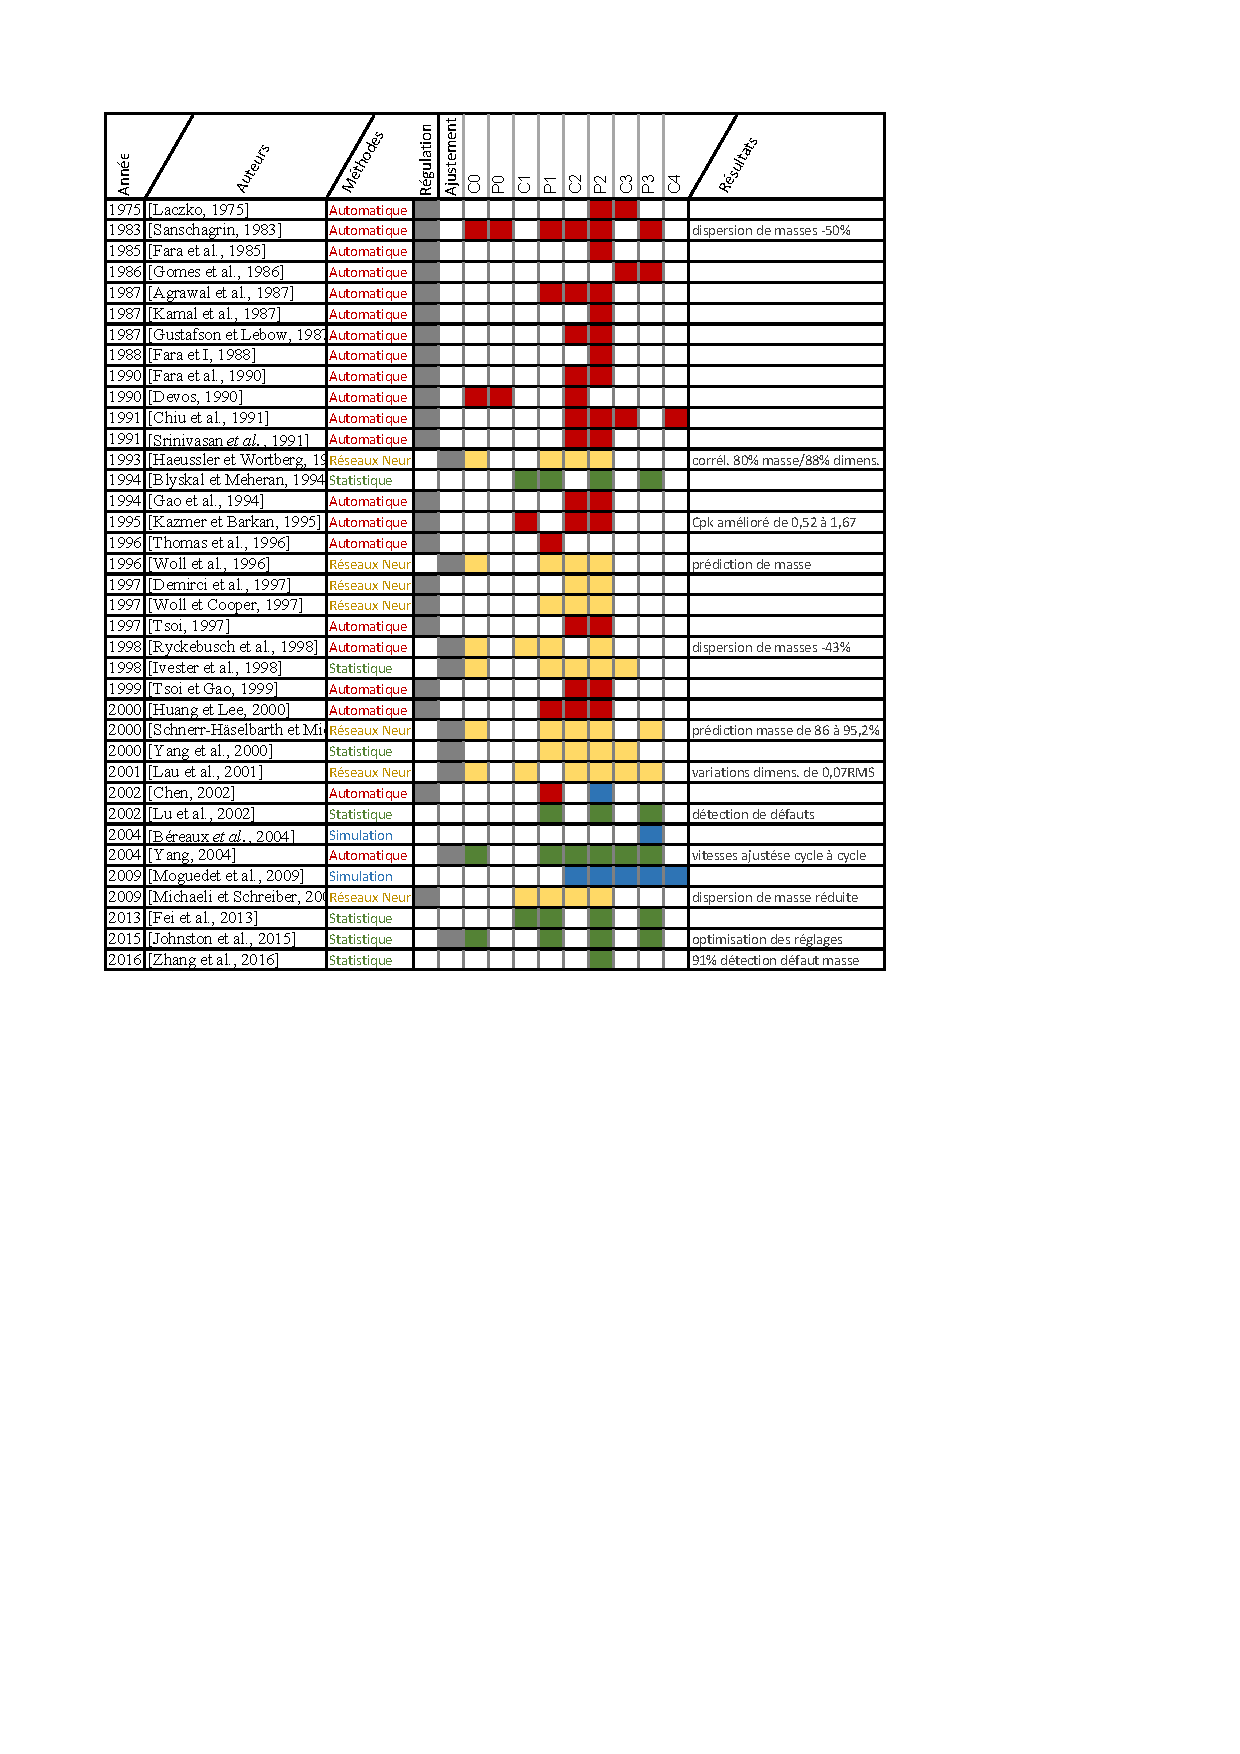
\includegraphics[width=\textwidth,height=\textheight,keepaspectratio]{../Chap1/Figures/TableauComparaisonEssais.pdf}
%	\caption{Cartographie bibliographique de la maîtrise du procédé d'injection-moulage.}
%	\label{tab:state_art_compare}
%\end{figure}

% from https://tex.stackexchange.com/a/416169
% \newcommand{\STAB}[1]{\begin{tabular}{@{}r@{}}#1\end{tabular}}
\newcommand{\bcline}[1]{\arrayrulecolor{black}\cline{#1}\arrayrulecolor{black}}
\begin{table}[hbtp]
	\centering
	\resizebox{\textwidth}{!}{%
		\begin{tabular}{!{\color{black}\vrule}l l l l!{\color{black}\vrule}l!{\color{gray}\vrule}l!{\color{gray}\vrule}l!{\color{gray}\vrule}l!{\color{gray}\vrule}l!{\color{gray}\vrule}l!{\color{gray}\vrule}l!{\color{gray}\vrule}l!{\color{gray}\vrule}l!{\color{black}\vrule}}
			\bcline{5-13} \multicolumn{1}{l}{} &                                &                                           &                                & \rotatebox[origin=r]{90}{Caractéristiques de la pièce stable} & \rotatebox[origin=r]{90}{Paramètres de stabilisation} & \rotatebox[origin=r]{90}{Caractéristiques de la pièce chaude} & \rotatebox[origin=r]{90}{Param. de maintien-refroidissement} & \rotatebox[origin=r]{90}{Caractéristiques de la pièce injectée} & \rotatebox[origin=r]{90}{Paramètres d'injection} & \rotatebox[origin=r]{90}{Caractéristiques de la matière fondue} & \rotatebox[origin=r]{90}{Paramètres de plastification} & \rotatebox[origin=r]{90}{Caractéristiques de la matière initiale} \\ \bcline{1-4}
			\multicolumn{1}{!{\color{black}\vrule}l!{\color{black}\vrule}}{Année} & \multicolumn{1}{l!{\color{black}\vrule}}{Auteurs [Publication]}   & \multicolumn{1}{l!{\color{black}\vrule}}{Méthode utilisée}     & \multicolumn{1}{l!{\color{black}\vrule}}{Objectif}       & $\boldsymbol{C}_0$                              & $\boldsymbol{P}_1$                              & $\boldsymbol{C}_1$       & $\boldsymbol{P}_2$       & $\boldsymbol{C}_2$       & $\boldsymbol{P}_3$                              & $\boldsymbol{C}_3$       & $\boldsymbol{P}_4$       & $\boldsymbol{C}_4$       \\ \bcline{1-13}
			1975                        & \citeauthor{laczko_controller_1975} \cite{laczko_controller_1975}                         & {\color[HTML]{CB0000} Automatique}        & {\color[HTML]{CE6301} Régulation}   &                                                 &                                                 &                          &                          &                          & \cellcolor[HTML]{CB0000}                        & \cellcolor[HTML]{CB0000} &                          &                          \\
			1983                        & \citeauthor{sanschagrin_process_1983} \cite{sanschagrin_process_1983}                    & {\color[HTML]{CB0000} Automatique}        & {\color[HTML]{CE6301} Régulation}   & \cellcolor[HTML]{CB0000}                        & \cellcolor[HTML]{CB0000}                        &                          & \cellcolor[HTML]{CB0000} & \cellcolor[HTML]{CB0000} & \cellcolor[HTML]{CB0000}                        &                          & \cellcolor[HTML]{CB0000} &                          \\
			1985                        & \citeauthor{fara_evaluation_1985} \cite{fara_evaluation_1985} & {\color[HTML]{CB0000} Automatique}        & {\color[HTML]{CE6301} Régulation}   &                                                 &                                                 &                          &                          &                          & \cellcolor[HTML]{CB0000}                        &                          &                          &                          \\
			1986                        & \citeauthor{gomes_injection_1986} \cite{gomes_injection_1986} & {\color[HTML]{CB0000} Automatique}        & {\color[HTML]{CE6301} Régulation}   &                                                 &                                                 &                          &                          &                          &                                                 & \cellcolor[HTML]{CB0000} & \cellcolor[HTML]{CB0000} &                          \\
			1987                        & \citeauthor{agrawal_injection-molding_1987} \cite{agrawal_injection-molding_1987} & {\color[HTML]{CB0000} Automatique}        & {\color[HTML]{CE6301} Régulation}   &                                                 &                                                 &                          & \cellcolor[HTML]{CB0000} & \cellcolor[HTML]{CB0000} & \cellcolor[HTML]{CB0000}                        &                          &                          &                          \\
			1987                        & \citeauthor{kamal_dynamics_1987} \cite{kamal_dynamics_1987} & {\color[HTML]{CB0000} Automatique}        & {\color[HTML]{CE6301} Régulation}   &                                                 &                                                 &                          &                          &                          & \cellcolor[HTML]{CB0000}                        &                          &                          &                          \\
			1987                        & \citeauthor{gustafson_model_1987} \cite{gustafson_model_1987} & {\color[HTML]{CB0000} Automatique}        & {\color[HTML]{CE6301} Régulation}   &                                                 &                                                 &                          &                          & \cellcolor[HTML]{CB0000} & \cellcolor[HTML]{CB0000}                        &                          &                          &                          \\
			1988                        & \citeauthor{fara_control_1988} \cite{fara_control_1988}                        & {\color[HTML]{CB0000} Automatique}        & {\color[HTML]{CE6301} Régulation}   &                                                 &                                                 &                          &                          &                          & \cellcolor[HTML]{CB0000}                        &                          &                          &                          \\
			1990                        & \citeauthor{fara_comprehensive_1990} \cite{fara_comprehensive_1990}                & {\color[HTML]{CB0000} Automatique}        & {\color[HTML]{CE6301} Régulation}   &                                                 &                                                 &                          &                          & \cellcolor[HTML]{CB0000} & \cellcolor[HTML]{CB0000}                        &                          &                          &                          \\
			1990                        & \citeauthor{devos_contribution_1990} \cite{devos_contribution_1990} & {\color[HTML]{CB0000} Automatique}        & {\color[HTML]{CE6301} Régulation}   & \cellcolor[HTML]{CB0000}{\color[HTML]{000000} } & \cellcolor[HTML]{CB0000}{\color[HTML]{000000} } &                          &                          & \cellcolor[HTML]{CB0000} &                                                 &                          &                          &                          \\
			1991                        & \citeauthor{chiu_dynamic_1991} \cite{chiu_dynamic_1991} & {\color[HTML]{CB0000} Automatique}        & {\color[HTML]{CE6301} Régulation}   &                                                 &                                                 &                          &                          & \cellcolor[HTML]{CB0000} & \cellcolor[HTML]{CB0000}                        & \cellcolor[HTML]{CB0000} &                          & \cellcolor[HTML]{CB0000} \\
			1991                        & Srinivasan et al.              & {\color[HTML]{CB0000} Automatique}        & {\color[HTML]{CE6301} Régulation}   &                                                 &                                                 &                          &                          & \cellcolor[HTML]{CB0000} & \cellcolor[HTML]{CB0000}                        &                          &                          &                          \\
			1993                        & \citeauthor{haeussler_quality_1993} \cite{haeussler_quality_1993} & {\color[HTML]{00009B} Réseau de Neurones} & {\color[HTML]{6200C9} Surveillance} & \cellcolor[HTML]{00009B}                        &                                                 &                          & \cellcolor[HTML]{00009B} & \cellcolor[HTML]{00009B} & \cellcolor[HTML]{00009B}                        &                          &                          &                          \\
			1994                        & \citeauthor{blyskal_applying_1994} \cite{blyskal_applying_1994} & {\color[HTML]{009901} Plan d'expériences} & {\color[HTML]{34696D} Pilotage}     &                                                 &                                                 & \cellcolor[HTML]{009901} & \cellcolor[HTML]{009901} &                          & \cellcolor[HTML]{009901}{\color[HTML]{000000} } &                          & \cellcolor[HTML]{009901} &                          \\
			1994                        & Gao et al.                     & {\color[HTML]{CB0000} Automatique}        & {\color[HTML]{CE6301} Régulation}   &                                                 &                                                 &                          &                          & \cellcolor[HTML]{CB0000} & \cellcolor[HTML]{CB0000}                        &                          &                          &                          \\
			1995                        & \citeauthor{kazmer_dynamic_1995} \cite{kazmer_dynamic_1995} & {\color[HTML]{CB0000} Automatique}        & {\color[HTML]{CE6301} Régulation}   &                                                 &                                                 & \cellcolor[HTML]{CB0000} &                          & \cellcolor[HTML]{CB0000} & \cellcolor[HTML]{CB0000}                        &                          &                          &                          \\
			1996                        & Thomas et al.                  & {\color[HTML]{CB0000} Automatique}        & {\color[HTML]{CE6301} Régulation}   &                                                 &                                                 &                          & \cellcolor[HTML]{CB0000} &                          &                                                 &                          &                          &                          \\
			1996                        & \citeauthor{woll_online_1996} \cite{woll_online_1996} & {\color[HTML]{00009B} Réseau de Neurones} & {\color[HTML]{6200C9} Surveillance} & \cellcolor[HTML]{00009B}                        &                                                 &                          & \cellcolor[HTML]{00009B} & \cellcolor[HTML]{00009B} & \cellcolor[HTML]{00009B}                        &                          &                          &                          \\
			1997                        & \citeauthor{demirci_numerical_1997} \cite{demirci_numerical_1997} & {\color[HTML]{00009B} Réseau de Neurones} & {\color[HTML]{CE6301} Régulation}   &                                                 &                                                 &                          &                          & \cellcolor[HTML]{00009B} & \cellcolor[HTML]{00009B}                        &                          &                          &                          \\
			1997                        & \citeauthor{woll_pattern-based_1997} \cite{woll_pattern-based_1997} & {\color[HTML]{00009B} Réseau de Neurones} & {\color[HTML]{CE6301} Régulation}   &                                                 &                                                 &                          & \cellcolor[HTML]{00009B} & \cellcolor[HTML]{00009B} & \cellcolor[HTML]{00009B}                        &                          &                          &                          \\
			1997                        & \cite{tsoi_fuzzy_1997} \citeauthor{tsoi_fuzzy_1997} & {\color[HTML]{CB0000} Automatique}        & {\color[HTML]{CE6301} Régulation}   &                                                 &                                                 &                          &                          & \cellcolor[HTML]{CB0000} & \cellcolor[HTML]{CB0000}                        &                          &                          &                          \\
			1998                        & Ryckebusch et al.              & {\color[HTML]{CB0000} Automatique}        & {\color[HTML]{CE6301} Régulation}   & \cellcolor[HTML]{CB0000}                        &                                                 & \cellcolor[HTML]{CB0000} & \cellcolor[HTML]{CB0000} &                          & \cellcolor[HTML]{CB0000}                        &                          &                          &                          \\
			1998                        & \citeauthor{ivester_automatic_1998} \cite{ivester_automatic_1998} & {\color[HTML]{009901} Plan d'expériences} & {\color[HTML]{6200C9} Surveillance} & \cellcolor[HTML]{009901}                        &                                                 &                          & \cellcolor[HTML]{009901} & \cellcolor[HTML]{009901} & \cellcolor[HTML]{009901}                        & \cellcolor[HTML]{009901} &                          &                          \\
			1999                        & \citeauthor{tsoi_real-time_1997} \cite{tsoi_real-time_1997} & {\color[HTML]{CB0000} Automatique}        & {\color[HTML]{CE6301} Régulation}   &                                                 &                                                 &                          &                          & \cellcolor[HTML]{CB0000} & \cellcolor[HTML]{CB0000}                        &                          &                          &                          \\
			2000                        & \citeauthor{huang_fuzzy_2000} \cite{huang_fuzzy_2000}                   & {\color[HTML]{CB0000} Automatique}        & {\color[HTML]{CE6301} Régulation}   &                                                 &                                                 &                          & \cellcolor[HTML]{CB0000} & \cellcolor[HTML]{CB0000} & \cellcolor[HTML]{CB0000}                        &                          &                          &                          \\
			2000                        & \citeauthor{schnerr-haselbarth_automation_2000} \cite{schnerr-haselbarth_automation_2000} & {\color[HTML]{00009B} Réseau de Neurones} & {\color[HTML]{6200C9} Surveillance} & \cellcolor[HTML]{00009B}                        &                                                 &                          & \cellcolor[HTML]{00009B} & \cellcolor[HTML]{00009B} & \cellcolor[HTML]{00009B}                        &                          & \cellcolor[HTML]{00009B} &                          \\
			2000                        & \citeauthor{yang_knowledgebased_2000} \cite{yang_knowledgebased_2000} & {\color[HTML]{009901} Plan d'expériences} & {\color[HTML]{6200C9} Surveillance} &                                                 &                                                 &                          & \cellcolor[HTML]{009901} & \cellcolor[HTML]{009901} & \cellcolor[HTML]{009901}                        & \cellcolor[HTML]{009901} &                          &                          \\
			2001                        & \citeauthor{lau_neural_2001} \cite{lau_neural_2001} & {\color[HTML]{00009B} Réseau de Neurones} & {\color[HTML]{6200C9} Surveillance} & \cellcolor[HTML]{00009B}                        &                                                 & \cellcolor[HTML]{00009B} &                          & \cellcolor[HTML]{00009B} & \cellcolor[HTML]{00009B}                        & \cellcolor[HTML]{00009B} & \cellcolor[HTML]{00009B} &                          \\
			2002                        & \citeauthor{chen_study_2002} \cite{chen_study_2002} & {\color[HTML]{CB0000} Automatique}        & {\color[HTML]{CE6301} Régulation}   &                                                 &                                                 &                          & \cellcolor[HTML]{CB0000} &                          & \cellcolor[HTML]{CB0000}                        &                          &                          &                          \\
			2003                        & \citeauthor{pillet_maitrise_2003} \cite{pillet_maitrise_2003} & {\color[HTML]{009901} MSP}                & {\color[HTML]{6200C9} Surveillance} &                                                 &                                                 & \cellcolor[HTML]{009901} & \cellcolor[HTML]{009901} & \cellcolor[HTML]{009901} & \cellcolor[HTML]{009901}                        &                          &                          &                          \\
			2004                        & \citeauthor{lu_stagebased_2004} \cite{lu_stagebased_2004} & {\color[HTML]{009901} Plan d'expériences} & {\color[HTML]{6200C9} Surveillance} &                                                 &                                                 &                          & \cellcolor[HTML]{009901} &                          & \cellcolor[HTML]{009901}                        &                          & \cellcolor[HTML]{009901} &                          \\
			2004                        & \citeauthor{yang_injection_2004} \cite{yang_injection_2004} & {\color[HTML]{CB0000} Automatique}        & {\color[HTML]{6200C9} Surveillance} & \cellcolor[HTML]{CB0000}                        &                                                 &                          & \cellcolor[HTML]{CB0000} & \cellcolor[HTML]{CB0000} & \cellcolor[HTML]{CB0000}                        & \cellcolor[HTML]{CB0000} & \cellcolor[HTML]{CB0000} &                          \\
			2006                        & \citeauthor{fournier_conduite_2006} \cite{fournier_conduite_2006} & {\color[HTML]{CB0000} Automatique}        & {\color[HTML]{34696D} Pilotage}     & \cellcolor[HTML]{CB0000}                        &                                                 & \cellcolor[HTML]{CB0000} & \cellcolor[HTML]{CB0000} &                          & \cellcolor[HTML]{CB0000}                        &                          &                          &                          \\
			2009                        & \citeauthor{michaeli_online_2009} \cite{michaeli_online_2009} & {\color[HTML]{00009B} Réseau de Neurones} & {\color[HTML]{CE6301} Régulation}   &                                                 &                                                 & \cellcolor[HTML]{00009B} & \cellcolor[HTML]{00009B} & \cellcolor[HTML]{00009B} & \cellcolor[HTML]{00009B}                        &                          &                          &                          \\
			2013                        & \citeauthor{fei_practical_2013} \cite{fei_practical_2013} & {\color[HTML]{009901} Plan d'expériences} & {\color[HTML]{6200C9} Surveillance} &                                                 &                                                 & \cellcolor[HTML]{009901} & \cellcolor[HTML]{009901} &                          & \cellcolor[HTML]{009901}                        &                          & \cellcolor[HTML]{009901} &                          \\
			2014                        & Zhao et al.                    & {\color[HTML]{009901} MSP}                & {\color[HTML]{6200C9} Surveillance} &                                                 &                                                 &                          &                          &                          & \cellcolor[HTML]{009901}                        & \cellcolor[HTML]{009901} &                          &                          \\
			2015                        & \citeauthor{johnston_-line_2015} \cite{johnston_-line_2015} & {\color[HTML]{34696D} Pilotage} & {\color[HTML]{6200C9} Surveillance} & \cellcolor[HTML]{009901}                        &                                                 &                          & \cellcolor[HTML]{009901} &                          & \cellcolor[HTML]{009901}                        &                          & \cellcolor[HTML]{009901} &                          \\
			2016                        & \citeauthor{zhang_statistical_2016} \cite{zhang_statistical_2016} & {\color[HTML]{009901} MSP}                & {\color[HTML]{6200C9} Surveillance} &                                                 &                                                 &                          &                          &                          & \cellcolor[HTML]{009901}                        &                          &                          &                          \\
			2017                        & Zhou et al.                    & {\color[HTML]{CB0000} MSP \& Auto.}       & {\color[HTML]{34696D} Pilotage}     &                                                 &                                                 & \cellcolor[HTML]{CB0000} &                          &                          & \cellcolor[HTML]{CB0000}                        & \cellcolor[HTML]{CB0000} &                          &                          \\
			\bcline{1-13}
		\end{tabular}%
	}
	\caption{Récapitulatif de l'étude bibliographique, Annexe \ref{Ann:process_control}.}
	\label{tab:state_art_compare}
\end{table}

% \subsection{Contraintes de mise en œuvre du procédé d'injection-moulage}
% -> Réglage initial du point de fonctionnement difficle
% -> Peu de dérive du procédé, causes exceptionnelles de Shewart
% -> Pas ou peu de mesure de la qualité en ligne de production, pourquoi ? -> introduire notre travail

% TODO: mettre en annexe cette partie + présenter le tableau récapitulatif de notre étude -> justifier que pour maîtriser on a besoin de mesurer.
\noindent
L'Annexe \ref{Ann:process_control} propose une étude bibliographique des techniques employées afin de maîtriser le procédé d'injection-moulage.
Le Tableau \ref{tab:state_art_compare} récapitule cette revue de la littérature.
Pour chacune des publications, nous identifions les variables du procédé étudiées selon la représentation \textit{Zig-Zag} présentée dans la Figure \ref{fig:zigzag}, ainsi que les résultats obtenus.
On observe que les travaux de recherche initiaux utilisent l'automatique pour réguler le procédé.
Par la suite, 
Dernièrement, les travaux s'appuient principalement sur une démarche de Maîtrise Statistique des Procédés.  % et sur la simulation numérique.
% Le procédé d’injection possède plusieurs phases interdépendantes, mais la littérature ne s’intéresse pas à l’étude de l’ensemble des variables et paramètres du procédé.
% De nombreuses études présentées se focalisent sur une unique phase du procédé.
% Il a pourtant été montré que des corrélations entre les paramètres et les différentes phases existent.
% Les études de la littérature sont centrées sur les paramètres de la phase d’injection ($\boldsymbol{P_3}$).

À partir de l'étude de ces travaux et de notre connaissance de la pratique industrie de la plasturgie, nous identifions les trois principales contraintes de mise en œuvre du procédé d'injection-moulage :
\begin{itemize}
	\item le réglage initial du point de fonctionnement (paramètres $\boldsymbol{P_{2-4}}$),
	\item la surveillance des dérives des caractéristiques du procédé $\boldsymbol{C_{1-4}}$ et du produit $\boldsymbol{C_{0}}$.
	\item l'ajustement des réglages $\boldsymbol{P_{2-4}}$ pour modifier les caractéristiques du produit $\boldsymbol{C_{0}}$.
\end{itemize}

% \subsubsection{Réglage du point de fonctionnement}\mbox{} \\
Aujourd'hui, l'industrie de la plasturgie repose sur l'expérience du technicien-régleur pour définir le point de fonctionnement initial.
Il n'existe pas de méthodes de réglages automatique du point de fonctionnement, mais des systèmes d'assistance au réglage ont été proposés §\ref{subsubsec:initial_expert}.
La multitude de paramètres qui peuvent être ajustés sur le procédé rend difficile la découverte d'un point de fonctionnement permettant de produire une pièce conforme.
Aussi, le réglage initial de la presse à injecter est long.
Il est nécessaire d'ajuster chacun des paramètres $\boldsymbol{P_{2-4}}$ du procédé, pour que les variables intermédiaires $\boldsymbol{C_{1-4}}$ soient satisfaisantes, ainsi que les caractéristiques $\boldsymbol{C}_0$ du produit.
De plus, il est difficile pour un technicien régleur d'avoir une vue d'ensemble de la valeur des variables intermédiaires.
Dans la pratique, le réglage initial du point de fonctionnement est une opération itérative et empirique.
Enfin, nous remarquons qu'aucune des représentations du procédé d'injection-moulage ne traite des techniques d'injection multi-buses, qui sont pourtant courantes.
La complexité du réglage est alors largement augmentée, car les paramètres de chaque buse doivent être réglés.

De manière inverse, si l'on souhaite ajuster une caractéristique $\boldsymbol{C}_0$ du produit, il est difficile de prédire comment modifier les valeurs de réglage $\boldsymbol{P_{2-4}}$.
Cela est rendu d'autant plus compliqué par le fait que les caractéristiques de la pièce stable $\boldsymbol{C}_0$ ne sont connues que plusieurs heures après sa production.
% Présenter les contraintes du procédé d'injection

Dans le cadre de notre travail, nous proposons de dépasser cette limite en identifiant un modèle qui prédit les caractéristiques des pièces stables $\boldsymbol{C}_0$ à partir des caractéristiques des pièces en sortie de la machine $\boldsymbol{C_1}$.
Ce modèle sera construit par apprentissage statistique.
Dans le Chapitre \ref{ch:measure}, nous discuterons du mesurage des caractéristiques $\boldsymbol{C_1}$ des pièces chaudes, juste après la sortie du moule.
Puis dans le Chapitre \ref{ch:metric_learning}, nous discuterons de la construction d'un modèle de la qualité $\boldsymbol{C}_0$ des pièces par apprentissage statistique.

% La régulation du procédé d'injection est une thématique d'étude riche.
La régulation du procédé d'injection-moulage est le  sujet de nombreux travaux.
Les outillages modernes possèdent des capteurs qui permettent de connaître précisément les caractéristiques de la matière, telles que la pression ou la température dans le moule.
% Aussi, les modèles du procédé d'injection-moulage qui sont les plus avancés sont construits par l'expérience §\ref{parag:molding_doe}.
% Les plans d'expériences sont souvent utilisés dans les études.
La méthode qui est certainement la plus avancée est proposée en 2009.
\citeauthor{michaeli_online_2009} réalise la régulation des paramètres de l'ensemble des phases d'injection, de maintien et de refroidissement \cite{michaeli_online_2009}.
Cela permet de suivre le diagramme de transformation de la matière Pression, Volume, Température (PVT) idéal pendant l'ensemble du cycle §\ref{subsec:regulation}.
La difficulté de la régulation de toutes les variables $\boldsymbol{C_{2-3}}$ est due à la complexité de la modélisation du procédé, en particulier des interactions entre les variables.
Les auteurs de cette étude utilisent un modèle à réseau de neurones qui est identifié à partir des mesures de pression et de températures dans le moule pendant le cycle.
L'optimisation des paramètres à partir du modèle permet de trouver les ajustements qui permettent de suivre le diagramme PVT.
Les auteurs étudient l'effet de cette régulation du procédé sur la dispersion de la masse des pièces, lorsque la température du fourreau est modifié pour introduire une perturbation : la masse est stabilisée.
Il aurait été intéressant d'étudier d'autres caractéristiques de la pièce, comme par exemple la géométrie.

Enfin, la détection des dérives du procédé est un des objectifs de nos travaux.
En effet, nous souhaitons proposer un système de contrôle de la qualité en ligne de production.
L'analyse du résultat du contrôle permettra de détecter les dérives.
En 2003, \citeauthor{pillet_maitrise_2003} proposent des principes pour adapter la Maîtrise Statistique des Procédés à l'injection-moulage \cite{pillet_maitrise_2003}.
Le choix des variables à contrôler peut se faire sur les paramètres du procédé et sur les caractéristiques du produit.
Les auteurs recommandent de choisir peu de variables.
Celles-ci doivent être les plus représentatives possibles des défauts à surveiller.
Enfin, il est recommandé de choisir des variables faciles à mesurer.
Le procédé d'injection-moulage est capable de produire une pièce toutes les 30 secondes, c'est pourquoi le risque de faux positif est ajusté.
Ce risque est généralement défini à plus ou moins trois fois l'écart-type de la distribution de la valeur surveillée.
Dans le cas de l'injection, cela correspondrait à une fausse alarme toutes les 2,5 heures, soit $0,27\%$ de pièces hors-contrôles.
Cette fréquence est trop élevée, c'est pourquoi les auteurs recommandent d'ajuster le risque à 4,5 fois l'écart-type, soit $0,00068\%$ de pièces hors-contrôles, soit une pièce toutes les 992 heures de production.
Cette démarche diminue drastiquement l'intervalle de tolérance du procédé.
En cas de détection d'une situation hors-contrôle, il est recommandé d'écarter les pièces concernées.
En cas de répétition de cette situation hors-contrôle sur plusieurs pièces, il est recommandé d'arrêter la machine et de faire intervenir le technicien-régleur.

Une démarche complémentaire à la détection des dérives serait de réaliser un ajustement des paramètres du procédé pour compenser la dérive, c'est le "pilotage" du procédé.
Nous détaillerons l'apport de notre dispositif de  mesure en ligne de production pour le pilotage dans la Section suivante.

% Il sera alors envisageable d'ajuster les paramètres du procédé à partir de notre mesure de la qualité des produits.


% pouvoir proposer une modification des réglages adaptée.

%\subsection{Optimisation du procédé d'injection-moulage}
%En 2001, \citeauthor{thyregod_modelling_2001} définit le temps de refroidissement comme le facteur principal de la qualité et de la durée du temps de cycle, pour une production multi-empreintes \cite{thyregod_modelling_2001}.
%Il propose ainsi d'optimiser le ratio entre durée de la phase de refroidissement et profit économique réalisé par heure.
%Ce critère permet d'optimiser qualité et productivité.
%L’objectif est de réduire la durée des phases du cycle.
%La durée incompressible de la phase de dosage, réalisée en temps masqué, est la limite à cette optimisation.
%Les systèmes de canaux chauds (\textit{hot runner}) réduisent les durées d’injection et de refroidissement : les canaux de distribution de la matière sont maintenus à température par des éléments chauffants de sorte que la matière reste à l’état fondu dans les canaux pendant l’ensemble du cycle.
%Enfin, des moules à refroidissement actif, capable de dissiper rapidement la chaleur, réduisent la durée du refroidissement \cite{kazmer_towards_1999}.
%
%Dans la pratique industrielle, afin de minimiser les coûts d’immobilisation du stockage, on cherche à réduire au maximum le stockage entre les étapes.
%Les défauts géométriques et d’aspect apparaissent majoritairement lors des étapes de déplacements des pièces entre les étapes successives de la production.
%Pour des pièces techniques au cahier des charges rigoureux, un contrôle qualité avant expédition est donc obligatoire.
%Les défauts géométriques et d’aspect sont également produits lors de l’étape initiale d’injection-moulage.
%De nombreux défauts dit "d’aspect" sont des défauts géométriques à l’échelle de la centaine de micromètres.
%Ceux-ci modifient les réflexions des lumières incidentes et cause des changements de luminosité brusques, qui ne sont pas acceptables pour le cahier des charges du produit fini.
%Les étapes de peintures peuvent mettre en valeurs des défauts en introduisant des surfaces spéculaires.
%
%
%en comparaison du coût des étapes de finitions suivantes, telles que les étapes de peintures.
%Éviter aux pièces de mauvaise qualité d’être peintes est une priorité.
%En second temps, un système de rétroaction pourra être déployé sur le procédé, afin de maximiser la qualité produite.

\subsection{La mesure de la qualité du produit en ligne : un verrou technologique au pilotage automatique}
% TODO:
% Le pilotage du procédé d’injection-moulage des thermoplastiques est une thématique de recherche riche, aux enjeux industriels importants.
% Le pilotage peut s’appuyer sur de multiples méthodes issues de la théorie du contrôle, de la statistique ou de l’ajustement des procédés qui s’appuient sur une instrumentation de la machine.
% Le procédé d’injection possède des paramètres non-linéaires liés en valeurs et en temps.
% Dans ce sens, les capacités des réseaux de neurones à modéliser par apprentissage puis à répondre à un problème multi-entrées et multi-sorties sont mises en avant.

D'après le Tableau \ref{tab:state_art_compare}, le mesurage des caractéristiques qualité des produits, dès leurs sorties de l'outillage est peu étudiée.
% Il est nécessaire de définir les critères qualités des pièces.
La caractéristique la plus étudiée dans la littérature est la masse de la pièce \cite{schnerr-haselbarth_automation_2000, fournier_conduite_2006, michaeli_online_2009}.
Cela s'explique par la facilité de la réalisation de la pesée, dès la sortie de la machine, ainsi que par la bonne précision des balances.
Dans l'industrie, la masse est souvent considérée comme une caractéristique qui valide la qualité de la pièces.
Si les pièces ont des manques, la masse sera nécessairement plus faible.
De plus, la quantité de matière injectée fait varier la masse et fait également varier les caractéristiques mécaniques.
% Il y a aussi un lien entre le taux d'humidité de la matière et la masse des pièces.

Le contrôle qualité dimensionnel peut être automatisé par imagerie de profil.
% Il demande un équipement calibré et automatisé.
Il prend place après la production et il permet d'exclure les pièces non conformes.
% Ce contrôle dimensionnel ne s'intéresse pas à l'aspect des pièces, uniquement aux profils géométriques.
En pratique, il est généralement réalisé par un humain à l'aide d'un comparateur.
Le coût et la complexité de l'installation de l'imagerie de profil réserve cette méthode automatique aux productions à haute valeur ajoutée.

Nous remarquons que de nombreuses études annoncent réaliser le contrôle de la qualité du produit, alors qu'elles s'intéressent uniquement à la masse ou à une cotation géométrique.
En revanche, les caractéristiques d'aspects des pièces n'ont jamais été mesurées en ligne de production.
% La maîtrise de l'aspect dans les productions industrielles est une thématique de recherche importante. % alors que l'ensemble de la profession effectue des recherches et développements pour obtenir de meilleures qualités d'aspect.
Les cahiers des charges posent pourtant des contraintes en termes d'aspect : pas de trace, pas de tâche, une couleur uniforme, une texture définie.
Généralement, les mesures complémentaires de la qualité des produits, comme l'aspect, sont effectuées après de la production d'un lot, parfois plusieurs heures après la production.
Notre travail cherche à proposer une mesure des caractéristiques d'aspect des pièces pendant le cycle de production.

De plus, les caractéristiques d'aspect contiennent des informations importantes pour l'analyse des causes de la variabilité d'une pièce. % et intéressent le client.
Le technicien-régleur utilise prioritairement l'aspect des pièces pour régler la machine.
% Le manque de spécifications et la difficulté à mesurer en cycle, ont limité l'utilisation du mesurage des caractéristiques d'aspect.
Une perspective à long terme de nos travaux pourra être le pilotage automatique du procédé d'injection-moulage.
Pourtant, aucun système de pilotage automatique n'a aujourd'hui pris en compte les caractéristiques visuelles des pièces.
À l'aide de l'information recueillie par notre dispositif de contrôle sur les caractéristiques de la pièces, il pourrait être possible de proposer des ajustements des paramètres afin de modifier les caractéristiques de la pièce produite.

% Nous répondrons à la problématique de la spécification de la notion de qualité dans le Chapitre \ref{ch:measure}.
% Proposer un dispositif de contrôle de l'aspect des pièces, en ligne de production, permettra de piloter le procédé sur directement sur les attentes du cahier des charges.

% \begin{raggedright}
\section{Objectif de recherche : le contrôle qualité en ligne de production} \label{sec:research_objectives}
% \end{raggedright}
Le mesurage de la qualité du produit en ligne de production est nécessaire pour optimiser la qualité de la production.
À partir de la mesure et des spécifications du cahier des charges, nous pouvons réaliser le contrôle de la qualité.
% En étant réalisée de manière automatique au sein de la ligne de production, le contrôle de la qualité permet d'ajuster les réglages de la machine dès la pièce suivante.
Dans nos travaux, nous chercherons à proposer un dispositif de contrôle adapté aux contraintes industrielles.
Nous avons identifié trois verrous au déploiement massif du contrôle qualité à cent pour-cent sur les lignes de production :
\begin{description}
	\item[Économique] : c’est le coût du dispositif de mesure,
	\item[Technologique] : le respect des contraintes industrielles,
	\item[Humain] : la représentation de la notion de qualité à partir de l'expertise humaine.
\end{description}
Dans les sections suivantes, nous détaillerons chacune de ces limites.
L'objectif de notre travail sera de proposer une solution technique pour les dépasser.

% \begin{raggedright}
\subsection{Viabilité économique du déploiement du mesurage de la qualité en ligne de production}
% \end{raggedright}

\begin{figure}[hbt]
	\centering
	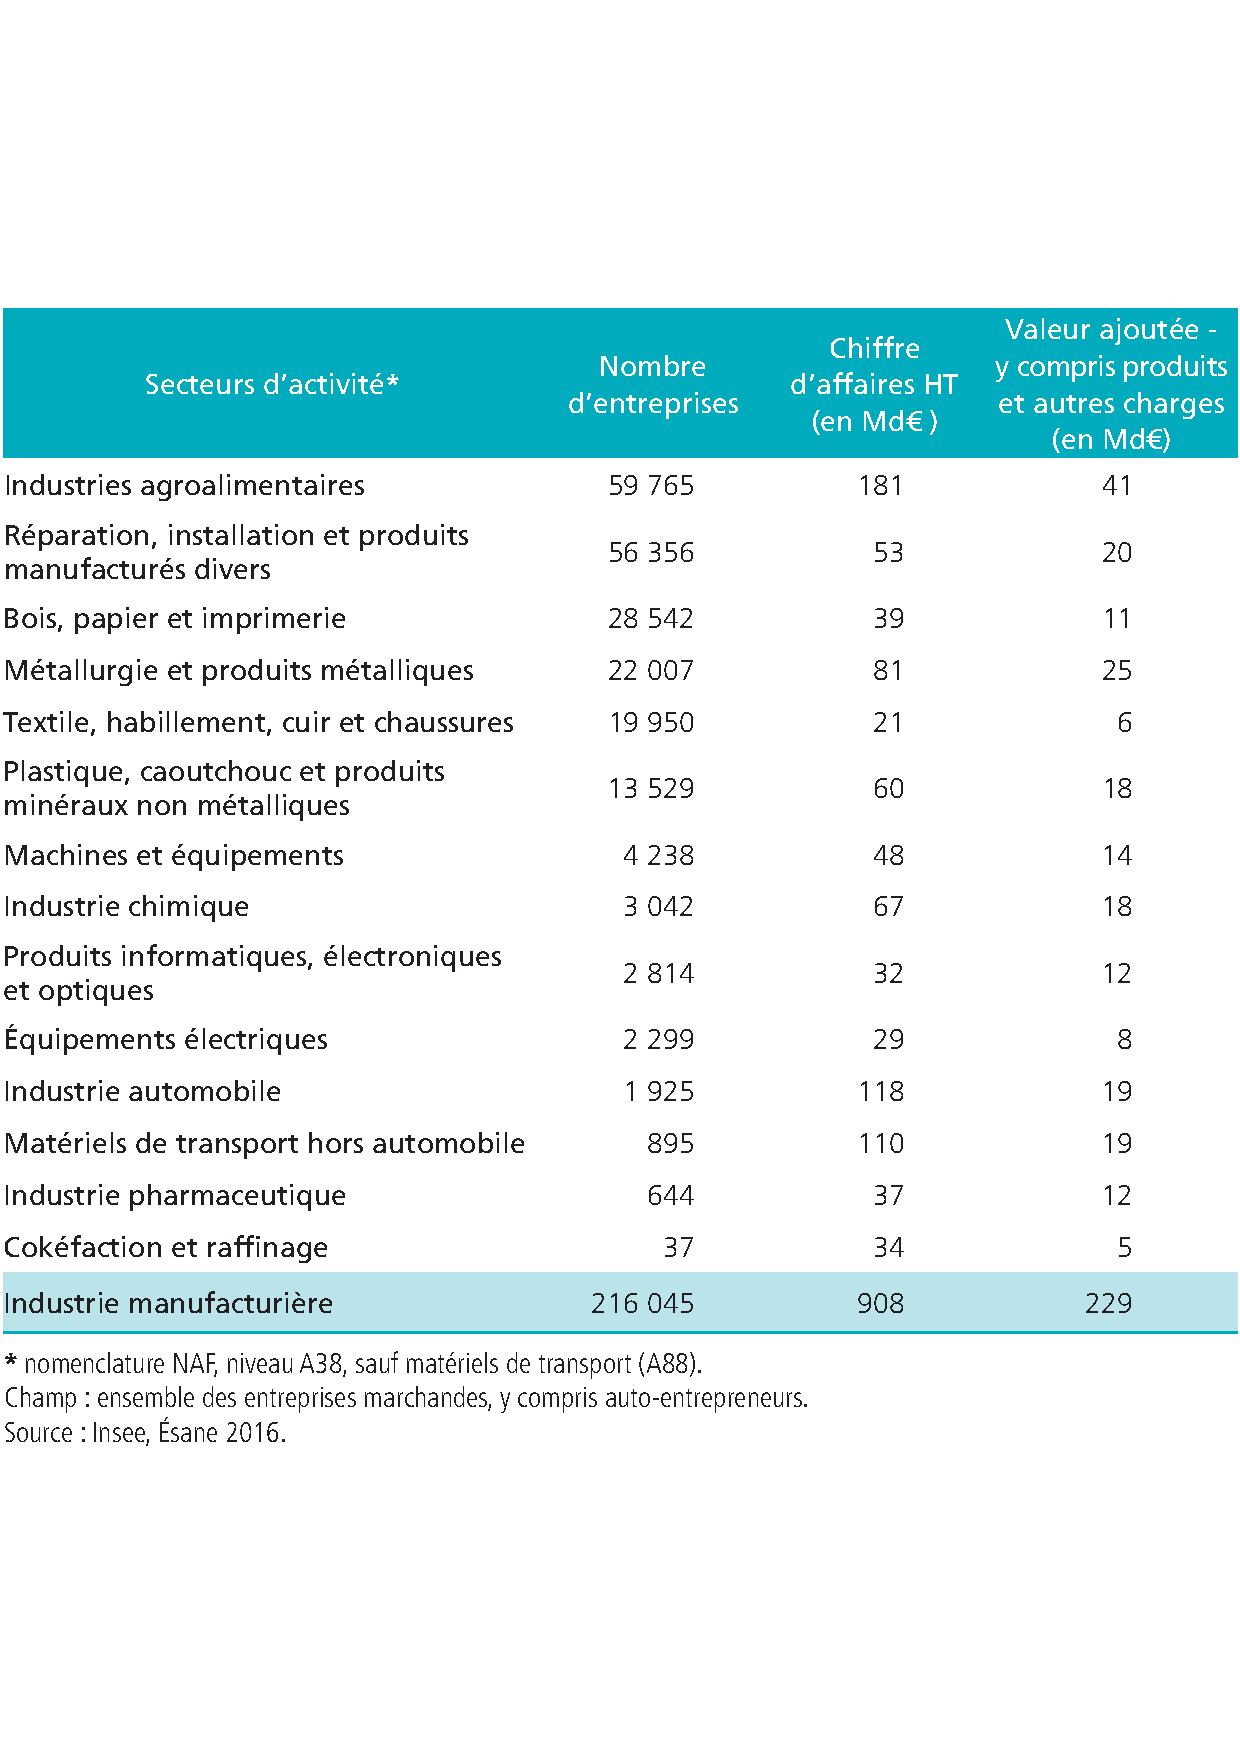
\includegraphics[width=0.85\textwidth,height=\textheight,keepaspectratio]{../Chap1/Figures/2018-Chiffres-cles-industrie-manufacturiere-secteur.pdf}
	\caption{Figure issue du rapport annuel de la \citeauthor{directiongeneraledesentreprises_chiffres_2019} :  \citetitle{directiongeneraledesentreprises_chiffres_2019} \cite{directiongeneraledesentreprises_chiffres_2019}}
	\label{fig:molding_economy}
\end{figure}

L'automatisation du contrôle des produits est principalement déployée pour des productions à gros volumes.
Les productions industrielles ont pour caractéristiques une cadence élevée (c'est à dire un temps de cycle court) et une marge sur le produit final généralement faible.
La Figure \ref{fig:molding_economy} indique une marge moyenne de 27\% pour le secteur de la plasturgie française, en 2016 \cite{directiongeneraledesentreprises_chiffres_2019}.
C'est une marge relativement élevée en comparaison des autres secteurs d'activé.
Le nombre d'entreprise du secteur est également important.
En estimant que 1\% de la marge du secteur de la plasturgie devrait être dépensé pour automatiser le contrôle de la qualité (soit 180 M€), on obtient un budget de 13 000€ par entreprise pour le contrôle qualité.
Cette estimation arbitraire permet de rendre compte du budget limité de l'automatisation du contrôle.
Contrairement à la transformation de la matière première, le contrôle de la qualité n'apporte pas de valeur au produit final ; c'est une sécurité pour respecter le cahier des charges et palier aux dérives du procédé.
% C'est pourquoi le coût d'intégration d'un dispositif de mesurage de la qualité se doit d'être faible.
% Le contrôle qualité à cent pour-cent présente un coût d'installation et de fonctionnement.
Il est nécessaire de définir les caractéristiques d'un système de mesure économiquement viable, pour les productions industrielles.

% Aller capter des infos qui sont porteuses de l'info de non-conformité mais qui ne sont pas directement la conformité finale.
% 7.2.1	Maitrise Statistique du Procédé (MSP/SPC)
% Les variations brutales peuvent être détectées par une analyse MSP/SPC des variables-machine en temps réel, mais les dérives faibles et lentes sont difficilement détectées.
% L’objectif de toute surveillance SPC est de détecter ces dérives le plus tôt possible pour éviter de produire. 
% La mesure par prélèvement de pièces, sur un procédé qui possède des étapes successives, ne permet pas d’identifier l’étape à l’origine du défaut.

\subsubsection{Intérêt économique du contrôle de la qualité en ligne de production}
Pour un produit qui nécessite un niveau de qualité très élevé, il est nécessaire de réaliser un contrôle qualité final de chaque pièce (contrôle à cent pour-cent).
Dans le cas de l'injection-moulage de pièces plastiques, le contrôle qualité final est souvent effectué plusieurs heures après l’étape de moulage.
Parfois, le contrôle final est réalisé après l’ajout de valeur des étapes de finitions.  %, ce qui prend parfois plusieurs jours.
Si la pièce est non-conforme juste après le moulage, alors de la valeur a été ajoutée à une pièce non-conforme.
De plus, la valeur ajoutée par les étapes de finitions, telles que la peinture ou la galvanoplastie, est bien plus important que la valeur ajouté par l'injection-moulage.
Si le temps de cycle du procédé permet de produire une pièce toutes les 30 secondes, ce qui correspond à milles pièces par journée de 8 heures.
Si le défaut de qualité est détecté un jour après son apparition, cela correspond à 1000 pièces rebuts qui ont été finies inutilement.
% Cette valeur peut être très important pour une production industrielle.
L’objectif du contrôle qualité en ligne est de détecter les dérives de la qualité le plus tôt possible, afin d'éviter de produire et d'écarter les pièces de la chaîne d'ajout de valeur.
% Dans un second temps, il pourrait être possible d'ajuster les paramètres du procédé pour corriger les dérives qualité.

% 2.1 Viabilité économique de la possession du dispositif de mesure
% Dans le cas de l’injection plastique, le coût de la matière première et de l’étape d’injection-moulage est très faible en comparaison du coût des étapes de finitions. 
Le moulage d'une pièce non-conforme a un coût négligeable en comparaison du coût des étapes de peinture et de finitions de cette pièce non-conforme.
Détecter les pièces mauvaises dès la sortie de la presse d’injection, afin de les écarter de la chaîne de production, permet de diminuer les rebuts finaux et de supprimer ainsi les coûts associés à leurs finitions.
Le coût économique du dispositif de mesure est à rapporter au coût économique des rebuts.
% Des industriels nous ont confirmés que le coût de la production de rebuts est faible en comparaison du coût de déploiement d’un dispositif de mesure sur chaque machine.
% Si le coût du système de mesure dépasse la dizaine de milliers d’euros, il n’est pas intéressant.
% Un coût élevé restera néanmoins intéressant à plus long terme, or nous cherchons à obtenir une adoption rapide.

\subsubsection{Mesure de variables du procédé ou mesure de la qualité du produit}
Dans cette section, nous discuterons de l'intérêt de la mesure direct des caractéristiques du produit, à contrario de la mesure de variables du procédé.

La méthode la plus utilisée pour étudier les dérives du procédé d'injection-moulage est de positionner des capteurs à l’intérieur de l'outillage, directement en contact avec la matière.
Une analyse multi-variée permet ensuite de détecter les dérives du procédé.
Les capteurs les plus répandus sont les sondes de températures et les sondes de pressions \cite{kurt_experimental_2009}.
% Les données de ces capteurs sont analysées par différentes méthodes non-supervisés (carte de contrôle [Min, 2003], Analyse en Composante Principale [Zhang et al., 2015]) afin de détecter les dérives qualité sur une production stabilisée. La construction de modèle par apprentissage supervisé a également été proposée [Zhou et al., 2018]. Des capteurs plus complexes [Chen et al., 2004] et multivariés [Kazmer et al., 2011] ont été proposés, puis validés [Gordon et al., 2017].
Le coût de l’instrumentation invasive des moules est élevé.
Intégrer les conduits nécessaires au passage des fils et connecteurs est compliqué sachant que les moules intègrent également des canaux de refroidissements indispensables au procédé.
Nous estimons que l’intégration de capteurs dans l'outillage représente un surcoût de vingt pour-cent de la conception et de la fabrication de l'outillage.  % , pour un coût initialement compris entre cinquante et cent mille euros.
De plus, les capteurs subissent de fortes contraintes ce qui peut limiter leur durée de vie.
La défaillance d'un capteur nécessite l'arrêt de la production car celui-ci est intégré à l'outillage.
% Mais nous avons surtout observé des défaillances dans les fils de connections, lors des manipulations des moules pour les changements de productions.

De plus, un capteur intégré à un outillage est associé un outillage, et donc à une unique pièce.
Il n'est pas viable de démonter l'instrumentation du capteur pour le positionner sur un autre outillage.
À contrario, un dispositif de mesure extérieur au procédé ne serait pas lié à un outillage.
Cela permettrait de contrôler la qualité quand le cahier des charges le nécessite, quel que soit la pièce produite.
L'installation du dispositif de mesurage devra être simple, d'une durée inférieure à une heure, pour que sa mobilité soit réelle.
Un tel dispositif de mesure s'inscrit dans la démarche de l'industrie agile, où les lignes de productions sont fréquemment reconfigurées, en fonction des besoins.

Enfin, le mesurage de la pièce permet d'obtenir une information pertinente sur sa qualité ; à la différence des mesures de variables dans le moule, qui ne sont que des indicateurs de la qualité.
Nous détaillerons l'intérêt du contrôle non-invasif de la qualité dans le Chapitre \ref{ch:measure}.

\subsection{Faisabilité technologique du mesurage de la qualité en ligne de production}
Pour identifier un modèle du procédé, il est nécessaire de réaliser des mesurages afin de connaître l'état de celui-ci à différents instants.  % discrets.
Afin de pouvoir analyser l'évolution du procédé, l'échantillonnage des mesures doit être supérieure au temps caractéristique d'évolution du procédé.
Dans le cas de l'injection-moulage, l'évolution à court-terme du procédé est souvent proche d'une dizaine de cycles de production, soit de 100 à 600 secondes.  % soit le temps de cycle du procédé
Dans le cadre de notre travail, nous choisissons de réaliser le contrôle de cent pourcent des pièces.
Le mesurage doit être réalisé pendant la durée du cycle d'injection-moulage.
% Aller capter des infos qui sont porteuses de l'info de non-conformité mais qui ne sont pas
Pour respecter cette contrainte, nous distinguons deux grands types de mesures :
\begin{itemize}
\item les mesures dites "invasives", qui nécessite l'installation de capteurs de grandeurs physiques à l'intérieur de l'outillage et de la presse,
\item les mesures "non-invasives", qui s'intéressent à la pièce produite dès qu'elle sort de l'outillage et à l'extérieur de la presse.
\end{itemize}

% Les capteurs dans le moule peuvent mesurer la pression, la température ou bien la vitesse de déplacement de la matière par effet Doppler.
% En 2019, les systèmes d'acquisition utilisés avec ces capteurs fonctionnent à une fréquence de 25 à 1000 Hertz.
% Ainsi, le nombre de valeurs discrètes mesurées pendant un cycle est de l'ordre de dix milles.

Les mesures "invasives" nécessitent un travail de conception de l'outillage compliqué.
L'outillage intègre des canaux de refroidissement et le câblage des capteurs doit être conçu pour les éviter.
C'est pourquoi, \citeauthor{gao_multivariate_2012} proposent un capteur qui communiquent sans connectivité filaire \cite{kazmer_feasibility_2011, gao_multivariate_2012}.
L'outillage en acier conducteur est une cage de Faraday idéale.
La communication radiofréquence  est impossible.
C'est pourquoi leur capteur utilise des ondes acoustiques pour communiquer.
L'alimentation en énergie est assurée en récupérant les variations de pressions créées lors du cycle l'injection.
Cependant, cette solution n'est pour l'instant pas commercialisée.

De plus, la maintenance des capteurs intégrés à l'outillage est compliquée.
Les capteurs sont fragiles et les contraintes physiques qui s'exercent sur eux lors du cycle d'injection sont élevées.
En particulier, nous avons observé pendant nos campagnes d'essais que les défaillances proviennent le plus souvent des câbles et non des capteurs eux-mêmes.
En cas de défaillance d'un capteur, c'est l'ensemble de l'outillage qui est immobilisé, ce qui impacte fortement la production industrielle.
À contrario, le mesurage des pièces, dès leur sortie de l'outillage, ne demande pas ce travail de conception avancée.
Le système de mesure non-invasif est éloigné des contraintes physiques du procédé d'injection-moulage, ce qui limite le besoin de maintenance.
% Un système de mesure avec des imageurs est positionné en sortie de moule afin de mesurer la pièce.
% L'objet de ces travaux de thèse est le développement d'un système de mesure non invasif de la qualité des pièces produites.
% Cette démarche s'inscrit dans une réduction des coûts de l'instrumentation des moules et dans une logique de mesure directe de la qualité géométrique et d'aspect visuel de la pièce au plus tôt dans la chaîne de production.

Pour être intégrée à la ligne de production, le mesurage doit être réalisé dans une durée inférieure au temps de cycle du procédé d'injection-moulage.
Cette contrainte permet de réaliser le contrôle de cent pour-cent des pièces.
Si la pièce doit être déplacée devant le moyen de mesure, la durée du convoyage doit également être inclue.

\begin{figure}[tbhp]
	\centering
	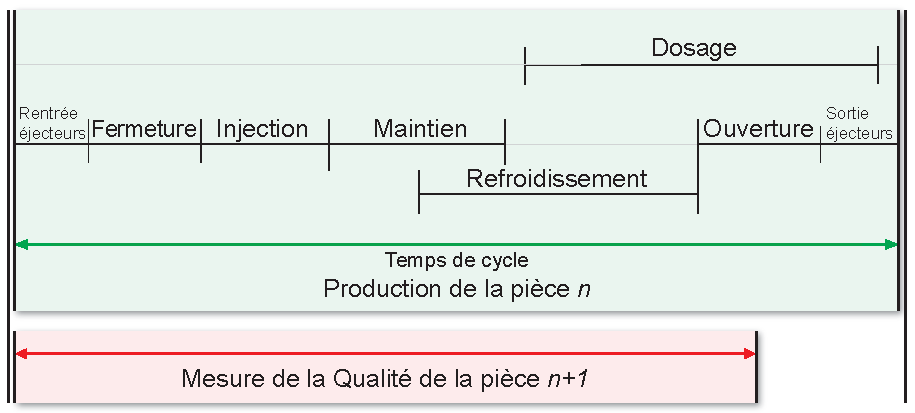
\includegraphics[width=0.82\textwidth,height=\textheight,keepaspectratio]{../Chap1/Figures/SAPRISTI_Chronogramme-Simple.pdf}
	\caption{Intégration de la mesure dans le cycle d'injection-moulage.}
	\label{fig:time_constraint}
\end{figure}

De plus, si on souhaite écarter la pièce non-conforme de la chaîne de production, il est alors nécessaire d'effectuer l'analyse de la mesure pendant la durée du cycle.
% Ces contraintes réduisent d'autant plus la durée disponible pour réaliser la mesure.
Nous estimons que la durée maximale de la mesure est de 10 secondes pour une durée du cycle de production de 60 secondes.
La Figure \ref{fig:time_constraint} inscrit la durée de la mesure dans le chronogramme du cycle du procédé (Figure \ref{fig:chronogramme}).
Cette contrainte de durée de la mesure sera une contrainte forte pour l'ensemble des choix technologiques de nos travaux.

Différentes mesures sont aujourd'hui compatibles, de par leurs courtes durées, avec une utilisation en cycle industriel : pesée de la masse ; imagerie par thermographie infrarouge ; contrôle d'aspect par caméras ; imagerie tridimensionnelle \cite{schwenke_optical_2002} ; durométrie ; imagerie des champs de contraintes par l'imagerie des phénomènes de photoélasticité sur les pièces plastiques transparentes.
% Pour obtenir des résultats fiables la mesure doit être automatisée.
% C'est un des objectifs de nos travaux.

La réalisation d'un système de mesure des caractéristiques des pièces dès la sortie du moule est un des objectifs de nos travaux.
Nous discuterons de manière approfondie des techniques de mesure existantes dans le Chapitre \ref{ch:measure}.

\subsection{Formalisation de la notion de qualité d'une pièce}
Le dispositif de contrôle de la qualité d'aspect le plus utilisé dans l'industrie de la plasturgie est l'humain.
\citeauthor{passaro_du_2014} s'appuie sur l'évaluation humaine structurée à l'aide d'un référentiel stricte pour déterminer la qualité de l'aspect de pièces plastiques \cite{passaro_du_2014}.

Aucune norme ne spécifie actuellement la notion qualité d'aspect.
Plusieurs travaux de recherche sont en cours, sur la notion de sensation tactile \cite{bruno_albert_formalisation_2016, albert_generic_2016, albert_smart_2017, albert_smart_2019, albert_maitrise_2019} et sur l'aspect visuel \cite{desage_syntactic_2015}.
Ces travaux associent une démarche de spécifications de la qualité, aux développements de nouveaux moyens de mesures \cite{desage_constraints_2015, pitard_metrologie_2016, lacombe_exploitation_2018a}.
Nos travaux s'inscrivent dans cette démarche de recherche.

Les pièces produites en injection-moulage des thermoplastiques possèdent une grande variété de dimension, de forme et d'état de surface.
Au sein d'une même entreprise, un système de contrôle de la qualité doit être capable de mesurer une grande variété de pièces.
Nous chercherons à simplifier au maximum l'utilisation de notre système de mesure afin de maximiser son adoption industrielle.   % , tout en répondant à la problématique du contrôle de la qualité en ligne de production.

La qualité d'aspect est une notion subjective qui est souvent définie dans les cahiers des charges sous la forme de défauthèques.
L'interprétation de ces définitions nécessite le travail d'un expert qualité humain.
L'expert qualité possède généralement la notion de la qualité du produit pour un atelier de production.
Il forme les opérateurs, afin de leur transmettre les exigences qui sont interprétées à partir du cahier des charges.
Cependant, il est difficile de transmettre ce savoir.
De plus, il est difficile d'obtenir une mesure répétable de la qualité par différents opérateurs.
Dans nos travaux, nous chercherons à automatiser cette interprétation.
Notre principal objectif de recherche est d'exploiter l'information issues des capteurs afin de proposer une mesure de la qualité d'aspect.
Notre système réalisera l'interprétation des mesures à partir d'un modèle de la qualité construit par apprentissage.
Cette démarche est détaillée dans le Chapitre \ref{ch:metric_learning}.
À terme, l'objectif est de proposer un modèle de la qualité qui serait générique à tous types de pièces ;
Ce modèle serait équivalent à un humain formé à l'expertise qualité ; il serait capable d'inspecter tous types de pièces et de détecter les défauts communs : manque de matière, retassure, brûlure.

% \subsection{Apprentissage statistique pour l'exploitation des mesures}
% L'exploitation des mesures multi-modales par un humain est compliqué.
% De plus, il est nécessaire d'adapter le système pour chaque pièce.
% Nous cherchons à proposer un système générique à toutes pièces.

\section{Conclusion}
Dans ce premier chapitre, nous avons présenté le contexte du procédé d'injection-moulage des thermoplastiques dans lequel s’inscrit ce travail de doctorat §\ref{sec:molding_presentation}.
Ce doctorat est également réalisé dans le cadre du projet de recherche collaboratif FUI SAPRISTI, qui cherche à optimiser le procédé d'injection-moulage.

Nous avons présenté dans la seconde partie les principaux enjeux de recherche sur le procédé d'injection-moulage §\ref{sec:research_topics}.
Une problématique de recherche importante est celle de la modélisation du procédé.
Nous proposons une représentation du procédé dans la Figure \ref{fig:zigzag}.
Cette représentation permet de mettre en évidence le nombre important de paramètres réglables et la nature séquentielle du procédé.
Nous identifions les paramètres réglables ainsi que les différentes caractéristiques de la matière au cours de sa transformation.

L'étude de la littérature montre l'intérêt porté à la recherche de modèles théoriques du procédé, à partir de la théorie physique.
Il s'agit de mieux comprendre les transformations physiques du polymère pendant son passage de granulés solides, fondue injectée, et pièce moulée solidifiée.

Une seconde thématique de recherche s'intéresse à l'identification de modèles empiriques.
Les études s'appuient sur les plans d'expériences pour réaliser les essais et sur les réseaux de neurones pour modéliser sous forme mathématique les non-linéarités du procédé.

Enfin, à partir d'une étude bibliographique (Annexe \ref{Ann:process_control}), nous présentons les principaux travaux sur la maîtrise du procédé d'injection-moulage.
Cela nous permet de mettre en évidence une limite importante de cette thématique : le manque de moyen de mesure en ligne de production des caractéristiques du produit.
Nous présentons l'intérêt de notre travail pour la maîtrise du procédé d'injection-moulage.

\smallskip

Dans le second partie de ce chapitre, nous avons présenter notre objectif de recherche.
Il s'agit de répondre au besoin de mesurage des caractéristiques du produit en ligne de production.
Nous mettons en évidence les principales contraintes industrielles.
Le coût du moyen de mesure doit être faible par rapport au coût de la production de pièces non-conformes.
Le mesurage doit être réalisé pendant la courte durée du cycle du procédé.
L'analyse de la mesure doit permettre de déterminer si la pièce est conforme ou non-conforme.

Le faible coût limitera l'emploi de certaines technologies de mesures.
Le contrôle de la qualité, si il est réalisé après l'étape de moulage de la pièce, permet d'écarter les pièces non-conformes de la chaîne de production.
L'économie réalisée est correspond à la valeur qui aurait été ajoutée à des pièces non-conformes lors des étapes suivantes de la chaîne de production.
Aujourd'hui, les mesures sur le procédé qui sont les plus répandues sont la pression et la température dans l'outillage.
Nous discutons de l'intérêt d'un moyen de mesure qui ne serait pas associé à un outillage.
Cela permettrait un positionnement de la mesure selon le besoin des chaînes de production.

Concernant la contrainte de durée de la mesure ; la durée d'un cycle d'injection est de 30 à 60 secondes.
Le faible coût requis du moyen de mesure, ainsi que la courte durée disponible limite le choix des capteurs.
Nous préférerons une mesure sans contact avec la pièce.
Nous discuterons des différentes technologies de mesure et des choix que nous avons effectués dans le Chapitre \ref{ch:measure}.

Enfin, il est nécessaire de réaliser le contrôle de la pièce à partir des mesures.
Cela nécessite d'interpréter le résultat de la mesure.
Dans le cadre des défauts géométriques, il existe des solutions de contrôle automatique.
Cependant, nous nous intéressons également dans le cadre de notre travail aux défauts d'aspect.
Aujourd'hui, l'expert qualité humain est requis pour interpréter l'aspect d'une pièce.
Un objectif de recherche concerne l'interprétation de la mesure et la formalisation de la notion de qualité d'aspect.
Nous présenterons les méthodes que nous avons retenues le Chapitre \ref{ch:metric_learning}.
Il s'agit de construire un modèle par apprentissage statistique qui détermine la qualité d'une pièce à partir des données de la mesure.
